% Combined presentation: Shubham, Swarali, Madhavi, Abhishek, Srinjoy.
% Uniform Madrid green, 8pt (latest supplied version). Reviewed 23 October 2026; 42 frames; continuous numbering.
% Replace the previous main.tex; keep the existing figures/ folder beside it.
% Compile with pdfLaTeX.
\documentclass[8pt,aspectratio=169]{beamer}
\usepackage[utf8]{inputenc}
\usepackage{amsmath,amssymb,mathtools,booktabs,array,graphicx,tikz,pgfplots}
\usepackage[most]{tcolorbox}
\usepackage{tabularx,colortbl}
\usetikzlibrary{arrows.meta,positioning,calc,shapes.geometric,shapes.symbols,decorations.pathreplacing,fit}
\pgfplotsset{compat=1.18}
\usetheme{Madrid}
\setbeamersize{text margin left=1em,text margin right=1em}
\renewcommand{\rmdefault}{cmr}
\renewcommand{\sfdefault}{cmss}
\renewcommand{\ttdefault}{cmtt}
\renewcommand{\encodingdefault}{OT1}
\renewcommand{\familydefault}{\sfdefault}
\renewcommand{\mathfamilydefault}{\sfdefault}

% Editable placeholders requested by the presenters; these are not verified repositories.
\newcommand{\CPSOurRepoURL}{https://github.com/your-team/cps-delay-attack}
\newcommand{\CPSOurDriveURL}{https://drive.google.com/drive/folders/project-folder-placeholder}
\gdef\CPSOrigin{PAPER}% PATCH: global so the footer sees it
\gdef\CPSSourceContext{}% PATCH
\gdef\CPSNoCtx{}% PATCH: empty-context marker for \ifx
\newcommand{\src}[1][]{\gdef\CPSSourceContext{#1}}% PATCH: \gdef, footer is typeset after the frame group closes
\newcommand{\chitest}{geometric ($\chi^2$) test}
\newcommand{\CPSCaption}[1]{\par\vspace{1mm}{\centering\scriptsize\color{black!65}#1\par}}
\newcommand{\CPSBaseSource}{Source: Nauta, Sandberg \& Maggio, \emph{Stealthy Computational Delay Attacks on Control Systems}, ICCPS 2025 \textperiodcentered{} \href{https://doi.org/10.1145/3716550.3722013}{DOI 10.1145/3716550.3722013}}
\newcommand{\CPSBaseOurs}{Our replay and analysis. Setting and code: Nauta, Sandberg \& Maggio, \emph{Stealthy Computational Delay Attacks on Control Systems}, ICCPS 2025}% PATCH
\newcommand{\CPSFootSource}{% PATCH: origin-aware, no dangling separator
  \def\CPSTmpOurs{OURS}%
  \ifx\CPSOrigin\CPSTmpOurs\CPSBaseOurs\else\CPSBaseSource\fi
  \ifx\CPSSourceContext\CPSNoCtx\else\ \textperiodcentered{} \CPSSourceContext\fi}

\makeatletter

% One Madrid green style for every teammate's section.
\definecolor{CPSgreen}{RGB}{0,110,60}
\newcommand{\CPSUniformStyle}{%
  \def\encodingdefault{OT1}\def\rmdefault{cmr}\def\sfdefault{cmss}\def\ttdefault{cmtt}%
  \def\familydefault{\sfdefault}\def\mathfamilydefault{\sfdefault}%
  \normalfont\normalsize
  \colorlet{madridgreen}{CPSgreen}%
  \colorlet{beamer@structure@color}{CPSgreen}%
  \colorlet{accent}{CPSgreen}\colorlet{accentlight}{CPSgreen!10}%
  \colorlet{slate}{CPSgreen!65!black}\colorlet{softgray}{CPSgreen!4}%
  \colorlet{navy}{CPSgreen!80!black}\colorlet{red}{CPSgreen!65!black}%
  \colorlet{teal}{CPSgreen}\colorlet{gold}{CPSgreen!70!black}%
  \colorlet{muted}{black!65}\colorlet{light}{CPSgreen!5}%
  \colorlet{amber}{CPSgreen}\colorlet{cream}{white}%
  \colorlet{ink}{CPSgreen!30!black}\colorlet{body}{black!80}%
  \colorlet{lorange}{CPSgreen!12}\colorlet{card}{white}%
  \colorlet{rule}{CPSgreen!35}\colorlet{chip}{CPSgreen!8}%
  \colorlet{hilite}{CPSgreen!14}\colorlet{head}{CPSgreen!18}%
  \colorlet{grey}{black!55}\colorlet{subt}{CPSgreen!10}%
  \colorlet{dia}{CPSgreen!7}\colorlet{forest}{CPSgreen}%
  \colorlet{deepgreen}{CPSgreen!70!black}%
  \setbeamercolor{structure}{fg=CPSgreen}%
  \setbeamercolor{normal text}{fg=black,bg=white}%
  \setbeamercolor{background canvas}{bg=white}%
  \setbeamercolor{frametitle}{fg=white,bg=CPSgreen}%
  \setbeamercolor{framesubtitle}{fg=white}%
  \setbeamercolor{block title}{fg=white,bg=CPSgreen}%
  \setbeamercolor{block body}{fg=black,bg=CPSgreen!5}%
  \setbeamercolor{block title alerted}{fg=white,bg=CPSgreen!65!black}%
  \setbeamercolor{block body alerted}{fg=black,bg=CPSgreen!5}%
  \setbeamercolor{block title example}{fg=white,bg=CPSgreen!80!black}%
  \setbeamercolor{block body example}{fg=black,bg=CPSgreen!5}%
  \setbeamerfont{frametitle}{size=\large,series=\bfseries}%
  \setbeamerfont{framesubtitle}{size=\small,shape=\upshape,series=\mdseries}%
  \setbeamerfont{block title}{size=\small,series=\bfseries}%
  \setbeamertemplate{navigation symbols}{}%
  \setbeamertemplate{headline}{}%
  \setbeamertemplate{blocks}[default]% flat blocks avoid opaque shadow-rendering artefacts
  \setbeamertemplate{footline}{%
    \begin{beamercolorbox}[wd=\paperwidth,sep=.6mm,leftskip=1.5mm,rightskip=1.5mm]{normal text}%
      \parbox[t][16pt][t]{\dimexpr\paperwidth-5mm\relax}{\fontsize{6}{7}\selectfont\color{black!65}\CPSFootSource}
    \end{beamercolorbox}%
    \hbox{%
      \begin{beamercolorbox}[wd=.13\paperwidth,ht=2.7ex,dp=1ex,center]{frametitle}%
        \fontsize{6}{7}\selectfont\bfseries\CPSOrigin
      \end{beamercolorbox}%
      \begin{beamercolorbox}[wd=.77\paperwidth,ht=2.7ex,dp=1ex,center]{frametitle}%
        \fontsize{6}{7}\selectfont Stealthy Computational Delay Attacks on Control Systems
      \end{beamercolorbox}%
      \begin{beamercolorbox}[wd=.1\paperwidth,ht=2.7ex,dp=1ex,right]{frametitle}%
        \fontsize{6.5}{7}\selectfont\insertframenumber\,/\,\inserttotalframenumber\hspace{2mm}%
      \end{beamercolorbox}}}%
  \@ifundefined{slidehead}{}{%
    \renewcommand{\slidehead}[3]{%
      \frametitle{##2}%
      \framesubtitle{##1}%
      {\small\color{black!80}##3\par}\vspace{.8ex}}}%
  \usebeamercolor[fg]{normal text}%
}

% Shared layout for the four speaker transitions.
\newcommand{\CPSSpeakerTitleContent}[5]{%
  \centering
  {\small\bfseries\color{CPSgreen}PRESENTATION PART #1\par}
  \vspace{1.2em}
  \begin{beamercolorbox}[wd=.94\linewidth,sep=12pt,center,rounded=true,shadow=false]{frametitle}
    {\LARGE\bfseries #2\par}
  \end{beamercolorbox}
  \vspace{1.1em}
  {\normalsize\bfseries\color{CPSgreen!75!black}#3\par}
  \vspace{.5em}
  {\small\color{black!75}#4\par}
  \vspace{1.7em}
  {\scriptsize\color{black!65}Presented by\par}
  \vspace{.3em}
  {\large\bfseries\color{CPSgreen}#5\par}
}

\makeatother
\begin{document}
% ==================== SHUBHAM (7 original frames)
\begingroup
\makeatletter



\definecolor{madridgreen}{RGB}{0,110,60}







% Shared colours, TikZ styles and figure macros.
% Used by delay_attacks_beamer.tex (the slides) and figures.tex (PNG export for the PowerPoint).

\definecolor{madridgreen}{RGB}{0,110,60}
\definecolor{hitgreen}{RGB}{46,160,90}
\definecolor{missred}{RGB}{200,40,40}
\definecolor{softgreen}{RGB}{228,242,233}
\definecolor{softred}{RGB}{250,228,228}
\definecolor{inkgray}{RGB}{90,90,90}



\tikzset{
  blk/.style={draw=madridgreen,very thick,rounded corners=3pt,fill=softgreen,minimum height=8mm,align=center,font=\small},
  arr/.style={-{Stealth[length=2.2mm]},very thick,draw=inkgray},
  hit/.style={draw=hitgreen!70!black,fill=hitgreen!80,minimum width=6mm,minimum height=5mm},
  miss/.style={draw=missred!70!black,fill=missred!85,minimum width=6mm,minimum height=5mm},
}

% ---------------------------------------------------------------- control loop
\newcommand{\FigLoop}{%
\begin{tikzpicture}[scale=0.95,transform shape]
  \node[blk,minimum width=3.4cm] (plant) at (0,2.6) {\textbf{Physical plant}\\[-1pt]{\scriptsize $x_{k+1}=Ax_k+Bu_k$}};
  \draw[dashed,thick,draw=inkgray,rounded corners=4pt,fill=gray!5] (-2.35,-1.55) rectangle (2.35,0.75);
  \node[font=\scriptsize\bfseries,text=inkgray,anchor=north west] at (-2.3,0.72) {Shared CPU};
  \node[blk,minimum width=2.2cm] (ctrl) at (-1.0,-0.25) {\textbf{Controller}\\[-1pt]{\scriptsize task, period $h$}};
  \node[draw=missred,very thick,rounded corners=3pt,fill=softred,align=center,font=\small,minimum height=8mm] (att) at (1.5,-0.25) {\textbf{Attacker}\\[-1pt]{\scriptsize CPU hog}};
  \draw[-{Stealth[length=2mm]},thick,missred] (att.west) -- (ctrl.east);
  \node[font=\tiny\bfseries,text=missred] at (0.33,-0.85) {starves};
  \draw[arr] (plant.west) -| (-2.75,-0.25) -- (ctrl.west);
  \node[font=\small,fill=white,inner sep=1pt] at (-2.75,1.3) {$y_k$};
  \node[font=\tiny,text=inkgray,fill=white,inner sep=1pt] at (-2.75,0.85) {sense};
  \draw[arr] (ctrl.south) |- (2.75,-1.95) -- (2.75,2.6) -- (plant.east);
  \node[font=\small,fill=white,inner sep=1pt] at (2.75,1.3) {$u_{k+1}$};
  \node[font=\tiny,text=inkgray,fill=white,inner sep=1pt] at (2.75,0.85) {actuate};
  \node[font=\tiny,text=inkgray,fill=white,inner sep=1pt] at (0.9,-1.95) {compute};
  \begin{scope}[shift={(0,-2.6)}]
    \draw[very thick,madridgreen,fill=white] (0,0) circle (0.38);
    \foreach \a in {0,30,...,330} \draw[madridgreen] (\a:0.30) -- (\a:0.36);
    \draw[very thick] (0,0) -- (90:0.25);
    \draw[very thick] (0,0) -- (20:0.18);
    \node[right=4mm,font=\scriptsize,align=left] at (0.1,0) {deadline every $h$};
  \end{scope}
\end{tikzpicture}}

% ---------------------------------------------------------------- taxonomy
\newcommand{\FigTaxonomy}{%
\begin{tikzpicture}[scale=0.92,transform shape,
  pt/.style={circle,fill=madridgreen,inner sep=1.6pt},
  lb/.style={font=\scriptsize}]
  \draw[-{Stealth},thick] (0,0) -- (0,2.7) node[above,font=\scriptsize\bfseries,align=center]{System\\knowledge};
  \draw[-{Stealth},thick] (0,0) -- (3.4,0) node[above,font=\scriptsize\bfseries,align=center,yshift=2pt]{Disruption\\resources};
  \draw[-{Stealth},thick] (0,0) -- (-1.7,-1.3) node[below,font=\scriptsize\bfseries,align=center]{Disclosure\\resources};
  \node[pt] at (-1.1,-0.85) {}; \node[lb,left] at (-1.15,-0.75) {Eavesdropping};
  \node[pt] at (1.5,0) {}; \node[lb,above] at (1.5,0.02) {DoS};
  \node[pt] at (0.9,-0.75) {}; \node[lb,right] at (0.95,-0.75) {Replay};
  \node[pt] at (1.6,1.3) {}; \node[lb,right] at (1.65,1.3) {Bias injection};
  \node[pt] at (1.0,2.0) {}; \node[lb,right] at (1.05,2.0) {Zero dynamics};
  \node[pt] at (0.9,0.85) {}; \node[lb,above left] at (0.95,0.85) {Covert};
  \node[star,star points=5,star point ratio=2.3,fill=missred,inner sep=1.4pt] at (2.6,0) {};
  \node[font=\scriptsize\bfseries,text=missred,below] at (2.6,-0.15) {Delay (new)};
\end{tikzpicture}}

% ---------------------------------------------------------------- attack timeline with hold / zero
\newcommand{\FigTimeline}{%
\begin{tikzpicture}[x=6.6mm,y=6.6mm]
  \node[font=\scriptsize\bfseries,anchor=east] at (-0.2,1.5) {Attack $a_i$};
  \node[font=\scriptsize\bfseries,anchor=east] at (-0.2,0.5) {Control job};
  \foreach \b [count=\i from 0] in {1,1,0,1,0,0,1,0} {
    \ifnum\b=1
      \node[font=\small\bfseries,text=missred] at (\i+0.5,1.5) {1};
      \node[miss] at (\i+0.5,0.5) {\textcolor{white}{\boldmath$\times$}};
    \else
      \node[font=\small\bfseries,text=hitgreen!70!black] at (\i+0.5,1.5) {0};
      \node[hit] at (\i+0.5,0.5) {\textcolor{white}{\checkmark}};
    \fi
  }
  \draw[-{Stealth},thick] (0,-0.2) -- (8.4,-0.2) node[right,font=\scriptsize]{$k$};
  \foreach \i in {0,...,8} \draw (\i,-0.3) -- (\i,-0.1);
  \begin{scope}[shift={(0,-3.1)}]
    \node[font=\scriptsize\bfseries,anchor=east] at (-0.2,1.0) {Hold: $u$};
    \fill[missred,opacity=0.12] (0,-0.1) rectangle (2,1.9) (3,-0.1) rectangle (4,1.9) (6,-0.1) rectangle (7,1.9);
    \draw[gray!50] (0,0) -- (8,0);
    \draw[ultra thick,madridgreen] (0,1.5) -- (2,1.5) -- (2,0.7) -- (4,0.7) -- (4,1.1) -- (5,1.1) -- (5,0.9) -- (7,0.9) -- (7,1.3) -- (8,1.3);
  \end{scope}
  \begin{scope}[shift={(0,-5.5)}]
    \node[font=\scriptsize\bfseries,anchor=east] at (-0.2,1.0) {Zero: $u$};
    \fill[missred,opacity=0.12] (0,-0.1) rectangle (2,1.9) (3,-0.1) rectangle (4,1.9) (6,-0.1) rectangle (7,1.9);
    \draw[gray!50] (0,0) -- (8,0);
    \draw[ultra thick,madridgreen] (0,0) -- (2,0) -- (2,0.7) -- (3,0.7) -- (3,0) -- (4,0) -- (4,1.1) -- (5,1.1) -- (5,0.9) -- (6,0.9) -- (6,0) -- (7,0) -- (7,1.3) -- (8,1.3);
    \node[font=\tiny,text=inkgray,anchor=north] at (4,-0.15) {shaded = missed period};
  \end{scope}
\end{tikzpicture}}

% ---------------------------------------------------------------- the three detector pictures
\newcommand{\FigWatchdog}{%
\begin{tikzpicture}[x=5.2mm,y=5.2mm]
  \foreach \b [count=\i from 0] in {0,1,0,1,1,1} {
    \ifnum\b=1 \node[miss,minimum width=4.6mm,minimum height=4.6mm] at (\i,0) {};
    \else \node[hit,minimum width=4.6mm,minimum height=4.6mm] at (\i,0) {}; \fi }
  \draw[decorate,decoration={brace,amplitude=4pt,mirror},thick] (2.6,-0.6) -- (5.4,-0.6);
  \node[font=\scriptsize\bfseries,text=missred] at (4,-1.4) {$\bar a$ in a row $\Rightarrow$ shutdown};
\end{tikzpicture}}

\newcommand{\FigWindow}{%
\begin{tikzpicture}[x=4.2mm,y=5.2mm]
  \foreach \b [count=\i from 0] in {0,0,1,0,1,0,1,1,0,0} {
    \ifnum\b=1 \node[miss,minimum width=3.6mm,minimum height=4.6mm] at (\i,0) {};
    \else \node[hit,minimum width=3.6mm,minimum height=4.6mm] at (\i,0) {}; \fi }
  \draw[madridgreen,ultra thick,rounded corners=2pt] (2.5,-0.6) rectangle (9.5,0.6);
  \node[font=\scriptsize\bfseries,text=madridgreen] at (6,-1.15) {last $n_w$ jobs};
\end{tikzpicture}}

\newcommand{\FigHistogram}{%
\begin{tikzpicture}[x=5.6mm,y=5.6mm]
  \draw[-{Stealth}] (-0.3,0) -- (4.3,0);
  \foreach \i/\e/\o in {0/2.2/2.1,1/1.1/1.0,2/0.55/0.7,3/0.28/0.5} {
    \fill[madridgreen!45] (\i,0) rectangle (\i+0.4,\e);
    \fill[missred!75] (\i+0.4,0) rectangle (\i+0.8,\o);
    \node[font=\tiny,below] at (\i+0.4,0) {\i};
  }
  \node[font=\tiny,anchor=north] at (2,-0.35) {burst length $i$};
  \node[font=\tiny,anchor=west] at (2.2,2.25) {\textcolor{madridgreen!45}{$\blacksquare$} expected};
  \node[font=\tiny,anchor=west] at (2.2,1.8) {\textcolor{missred!75}{$\blacksquare$} observed};
\end{tikzpicture}}

% ---------------------------------------------------------------- five-step icons (each about 1.6 x 1.1 cm)
\newcommand{\IconSetting}{%
\begin{tikzpicture}[x=1mm,y=1mm]
  \node[draw=madridgreen,thick,fill=softgreen,rounded corners=1pt,minimum width=9mm,minimum height=4.5mm,font=\tiny\bfseries] (p) at (0,6) {Plant};
  \node[draw=madridgreen,thick,fill=softgreen,rounded corners=1pt,minimum width=9mm,minimum height=4.5mm,font=\tiny\bfseries] (c) at (0,-1) {Ctrl};
  \draw[-{Stealth[length=1.2mm]},thick,inkgray] (p.west) -- ++(-3,0) |- (c.west);
  \draw[-{Stealth[length=1.2mm]},thick,inkgray] (c.east) -- ++(3,0) |- (p.east);
  \draw[very thick,madridgreen,fill=white] (11,-1) circle (2.2);
  \draw[thick] (11,-1) -- (11,0.6); \draw[thick] (11,-1) -- (12.1,-0.5);
\end{tikzpicture}}

\newcommand{\IconAttack}{%
\begin{tikzpicture}[x=1mm,y=1mm]
  \foreach \b [count=\i from 0] in {1,1,0,1,0} {
    \ifnum\b=1 \fill[missred!85] (\i*4.4,0) rectangle ++(3.8,3.8);
    \else \fill[hitgreen!80] (\i*4.4,0) rectangle ++(3.8,3.8); \fi }
  \node[draw=missred,thick,fill=softred,rounded corners=1pt,font=\tiny\bfseries,minimum width=12mm] at (10.8,8.5) {CPU hog};
  \draw[-{Stealth[length=1.2mm]},thick,missred] (10.8,6.6) -- (10.8,4.4);
\end{tikzpicture}}

\newcommand{\IconDetector}{%
\begin{tikzpicture}[x=1mm,y=1mm]
  \foreach \b [count=\i from 0] in {0,1,0,0,1,1,0} {
    \ifnum\b=1 \fill[missred!85] (\i*3.4,0) rectangle ++(2.9,3.6);
    \else \fill[hitgreen!80] (\i*3.4,0) rectangle ++(2.9,3.6); \fi }
  \draw[madridgreen,very thick,rounded corners=1pt] (6.4,-1) rectangle (24.2,4.6);
  \begin{scope}[shift={(12,10.5)}]
    \fill[madridgreen] (0,3.2) -- (3.2,2.2) -- (3.2,-0.4) .. controls (3.2,-2.6) .. (0,-3.6) .. controls (-3.2,-2.6) .. (-3.2,-0.4) -- (-3.2,2.2) -- cycle;
    \draw[white,very thick] (-1.4,-0.2) -- (-0.3,-1.4) -- (1.6,1.0);
  \end{scope}
\end{tikzpicture}}

\newcommand{\IconOptimise}{%
\begin{tikzpicture}[x=1mm,y=1mm]
  \draw[-{Stealth[length=1.2mm]},thick,inkgray] (0,0) -- (24,0);
  \draw[-{Stealth[length=1.2mm]},thick,inkgray] (0,0) -- (0,13);
  \draw[ultra thick,madridgreen] (1,1) .. controls (8,2) and (11,10) .. (15,10.5) .. controls (18,10.8) and (20,7) .. (23,5);
  \fill[missred] (15,10.5) circle (1.1);
  \node[font=\tiny\bfseries,text=missred,anchor=south] at (15,11.5) {max};
\end{tikzpicture}}

\newcommand{\IconPlants}{%
\begin{tikzpicture}[x=1mm,y=1mm]
  \foreach \x/\y/\h in {0/7/2.5,6/7/3.2,0/0/4,6/0/3} {
    \draw[thick] (\x,\y) rectangle ++(5,5.5);
    \fill[madridgreen!45] (\x+0.4,\y+0.4) rectangle ++(4.2,\h);
  }
  \begin{scope}[shift={(19,0)}]
    \fill[gray!30] (-4,-0.6) rectangle (4,0);
    \draw[thick,fill=gray!15] (-1.4,0) rectangle (1.4,4);
    \draw[line width=1.6pt,inkgray] (0,4.4) -- (5,5.4);
    \draw[line width=1.4pt,madridgreen] (5,5.4) -- (5.4,12);
    \fill[madridgreen] (5.4,12) circle (0.9);
  \end{scope}
\end{tikzpicture}}

% ---------------------------------------------------------------- the two test plants
\newcommand{\FigTank}{%
\begin{tikzpicture}[x=1cm,y=1cm,scale=0.62,transform shape]
  \foreach \x/\y/\h/\n in {0/1.6/0.5/3,1.6/1.6/0.65/4,0/0/0.8/1,1.6/0/0.6/2} {
    \draw[thick,fill=white] (\x,\y) rectangle (\x+1,\y+1.1);
    \fill[madridgreen!45] (\x+0.05,\y+0.05) rectangle (\x+0.95,\y+\h);
    \node[font=\scriptsize,text=inkgray] at (\x+0.5,\y+0.85) {\n};
  }
  \draw[thick,inkgray] (0.5,1.6) -- (0.5,1.1);
  \draw[thick,inkgray] (2.1,1.6) -- (2.1,1.1);
  \draw[thick,inkgray,-{Stealth[length=1.5mm]}] (-0.4,0.6) -- (-0.4,3.0) -- (2.3,3.0) -- (2.3,2.75);
  \draw[thick,inkgray,-{Stealth[length=1.5mm]}] (-0.4,0.6) -- (-0.4,-0.35) -- (0.3,-0.35) -- (0.3,-0.05);
  \draw[thick,madridgreen,-{Stealth[length=1.5mm]}] (3.0,0.6) -- (3.0,3.25) -- (0.3,3.25) -- (0.3,2.75);
  \draw[thick,madridgreen,-{Stealth[length=1.5mm]}] (3.0,0.6) -- (3.0,-0.35) -- (2.3,-0.35) -- (2.3,-0.05);
  \node[draw,circle,fill=white,inner sep=1.5pt,font=\tiny] at (-0.4,0.6) {P1};
  \node[draw,circle,fill=white,inner sep=1.5pt,font=\tiny] at (3.0,0.6) {P2};
\end{tikzpicture}}

\newcommand{\FigFuruta}{%
\begin{tikzpicture}[x=1cm,y=1cm,scale=0.62,transform shape]
  \fill[gray!25] (-1.4,-0.15) rectangle (1.4,0);
  \draw[thick,fill=gray!12,rounded corners=1pt] (-0.4,0) rectangle (0.4,1.0);
  \draw[thick,fill=gray!30] (0,1.12) ellipse (0.35 and 0.12);
  \draw[line width=3pt,inkgray,line cap=round] (0,1.15) -- (1.6,1.5);
  \draw[dashed,gray] (1.6,1.5) -- (1.6,3.2);
  \draw[line width=2.5pt,madridgreen,line cap=round] (1.6,1.5) -- (1.85,3.05);
  \fill[madridgreen] (1.85,3.05) circle (0.13);
  \draw[-{Stealth},thick,missred] (2.05,3.2) arc (75:25:0.9);
  \node[font=\scriptsize,text=missred,anchor=west] at (2.55,2.95) {falls};
  \draw[-{Stealth},thick,inkgray] (-0.75,0.6) arc (200:340:0.8 and 0.25);
  \node[font=\scriptsize,text=inkgray,anchor=east] at (-0.8,0.55) {motor};
\end{tikzpicture}}

% ---------------------------------------------------------------- defences watch the data, not the clock
\newcommand{\FigBlindSpot}{%
\begin{tikzpicture}[scale=0.95,transform shape]
  \node[blk,minimum width=3.0cm] (plant) at (0,1.9) {\textbf{Physical plant}};
  \node[blk,minimum width=3.0cm] (ctrl) at (0,0) {\textbf{Controller task}};
  \draw[arr] (plant.west) -- (-2.3,1.9) -- (-2.3,0) -- (ctrl.west);
  \draw[arr] (ctrl.east) -- (2.3,0) -- (2.3,1.9) -- (plant.east);
  \node[font=\small,fill=white,inner sep=1pt] at (-2.3,0.95) {$y_k$};
  \node[font=\small,fill=white,inner sep=1pt] at (2.3,0.95) {$u_{k+1}$};
  % physics-based detector watching the data
  \node[draw=madridgreen,very thick,rounded corners=3pt,fill=white,align=center,font=\scriptsize,minimum width=3.4cm] (det) at (0,3.45)
     {\textbf{Physics-based detector}\\ are $y$ and $u$ consistent with the model?};
  \draw[dashed,thick,madridgreen,-{Stealth[length=1.6mm]}] (-2.3,1.9) -- (-2.3,3.45) -- (det.west);
  \draw[dashed,thick,madridgreen,-{Stealth[length=1.6mm]}] (2.3,1.9) -- (2.3,3.45) -- (det.east);
  \node[circle,fill=hitgreen,text=white,font=\small\bfseries,inner sep=1pt] at (det.north east) {\checkmark};
  \node[font=\scriptsize\bfseries,text=madridgreen,anchor=south] at (0,3.95) {the data is watched};
  % the unwatched clock
  \begin{scope}[shift={(0,-1.45)}]
    \draw[dashed,thick,missred,rounded corners=4pt,fill=softred] (-2.3,-0.55) rectangle (2.3,0.55);
    \draw[very thick,missred,fill=white] (-1.4,0) circle (0.38);
    \foreach \a in {0,30,...,330} \draw[missred,shift={(-1.4,0)}] (\a:0.30) -- (\a:0.36);
    \draw[very thick,shift={(-1.4,0)}] (0,0) -- (90:0.25);
    \draw[very thick,shift={(-1.4,0)}] (0,0) -- (20:0.18);
    \node[font=\scriptsize\bfseries,text=missred,align=left,anchor=west] at (-0.8,0) {the \emph{timing} of $u$\\ is not watched};
  \end{scope}
  \draw[dashed,thick,missred] (0,-0.9) -- (ctrl.south);
\end{tikzpicture}}


% Footer: source line, then one green bar with the title and the page number (no presenter, no date).


\newcommand{\takeaway}[3]{%
  \noindent\begin{minipage}[t]{0.085\linewidth}\vspace{0pt}%
    \tikz\node[circle,fill=madridgreen,text=white,font=\small\bfseries,minimum size=5.5mm,inner sep=0pt]{#1};%
  \end{minipage}\hfill
  \begin{minipage}[t]{0.895\linewidth}\vspace{0pt}\raggedright
    {\color{madridgreen}\textbf{#2}}\\[0.1em]{\small #3}%
  \end{minipage}\par\vspace{0.75em}}

% One card of the "paper in five steps" slide: number, icon, title, section, text
\newcommand{\stepcard}[5]{%
  \begin{tikzpicture}
    \node[draw=madridgreen,thick,rounded corners=3pt,fill=white,minimum width=2.62cm,minimum height=4.3cm,anchor=north] (c) at (0,0) {};
    \fill[softgreen,rounded corners=3pt] ([xshift=0.6pt,yshift=-0.6pt]c.north west) rectangle ([xshift=-0.6pt,yshift=-1.75cm]c.north east);
    \node[circle,fill=madridgreen,text=white,font=\small\bfseries,inner sep=0pt,minimum size=5mm,draw=white,thick] at (c.north) {#1};
    \node at (0,-0.95) {\scalebox{0.9}{#2}};
    \node[anchor=north,font=\small\bfseries,text=madridgreen] at (0,-1.85) {#3};
    \node[anchor=north,font=\tiny,text=inkgray] at (0,-2.22) {#4};
    \node[anchor=north,text width=2.4cm,align=center,font=\footnotesize,execute at begin node={\hyphenpenalty=10000\relax}] at (0,-2.52) {#5};
  \end{tikzpicture}}

\title[Stealthy Computational Delay Attacks on Control Systems]{Stealthy Computational Delay Attacks\\ on Control Systems}
\subtitle{Talitha Nauta, Henrik Sandberg \& Martina Maggio \quad$\cdot$\quad ACM/IEEE ICCPS 2025}
\date{}


\def\CPSfootnote{}
\CPSUniformStyle
\beamer@calculateheadfoot
\makeatother


%===================================================================
\begin{frame}[c]
\gdef\CPSSourceContext{}
\gdef\CPSOrigin{PAPER}
\centering
\begin{beamercolorbox}[sep=10pt,center,rounded=true,shadow=false]{frametitle}
  {\Large\bfseries Stealthy Computational Delay Attacks\\on Control Systems\par}
  \vspace{.7em}
  {\small Talitha Nauta, Henrik Sandberg \& Martina Maggio\par}
  {\small ACM/IEEE ICCPS 2025\par}
\end{beamercolorbox}
\vspace{1.2em}
{\small\bfseries Embedded and Cyber-Physical Systems \textperiodcentered{} CS637\par}
\vspace{1em}
\renewcommand{\arraystretch}{1.5}
\begin{tabular}{>{\centering\arraybackslash}p{6.4cm}>{\centering\arraybackslash}p{6.4cm}}
\textbf{Shubham Tyagi} & \textbf{Swarali Nilesh Savale}\\[-.5em]
{\scriptsize Roll no.\ 20260001 (dummy)} & {\scriptsize Roll no.\ 20260002 (dummy)}\\
\textbf{Madhavi Singh} & \textbf{Abhishek Sharma}\\[-.5em]
{\scriptsize Roll no.\ 20260003 (dummy)} & {\scriptsize Roll no.\ 20260004 (dummy)}\\
\multicolumn{2}{c}{\textbf{Srinjoy Chakraborty}}\\[-.5em]
\multicolumn{2}{c}{{\scriptsize Roll no.\ 20260005 (dummy)}}
\end{tabular}\par% PATCH: end the paragraph so the date sits on its own line
\vspace{.8em}
{\small 22 October 2026\par}
\end{frame}

%===================================================================
\begin{frame}{Presentation plan}
\gdef\CPSSourceContext{}
\gdef\CPSOrigin{PAPER}
\centering
\begin{tikzpicture}[
  chev/.style={signal,signal to=east,signal from=west,minimum width=2.35cm,minimum height=1.1cm,
               draw=madridgreen,thick,fill=softgreen,text=madridgreen!70!black,font=\footnotesize\bfseries,align=center,inner sep=1pt},
  first/.style={chev,fill=madridgreen,text=white,draw=madridgreen},
  desc/.style={text width=2.1cm,align=center,execute at begin node={\hyphenpenalty=10000\relax},font=\scriptsize,text=black!80,anchor=north}]
  \foreach \t/\d [count=\i] in {
    {Introduction\\\& Brief}/{Why timing matters, the attack idea, key takeaways},
    {Problem\\Formulation}/{System model, switched dynamics, optimisation, detectors},
    {Paper's\\Results}/{The paper's two plants, figures and findings},
    {Our\\Reproduction}/{The authors' code and our reimplementation},
    {Defender\\Study}/{Policy replay and partial sweep},
    {Conclusion}/{Summary and references}} {
    \pgfmathsetmacro{\x}{(\i-1)*2.42}
    \ifnum\i=1 \node[first] (c\i) at (\x,0) {\t}; \else \node[chev] (c\i) at (\x,0) {\t}; \fi
    \node[circle,fill=white,draw=madridgreen,thick,font=\scriptsize\bfseries,text=madridgreen,inner sep=0pt,minimum size=4.6mm] at (\x,0.88) {\i};
    \node[desc] at (\x,-0.72) {\d};
  }
  \node[font=\scriptsize\bfseries,text=missred,anchor=south] at (0,1.18) {we start here};
\end{tikzpicture}

\note{The talk moves from the attack idea to the system model, then to the paper's evidence and our independent reproduction. We finish with policy replay, the defender-study formulation and the limitations of the partial sweep.}
\end{frame}

%===================================================================
\begin{frame}{Introduction: why timing is a security problem}
\gdef\CPSSourceContext{}
\gdef\CPSOrigin{PAPER}
\begin{columns}[T]
\begin{column}{0.50\textwidth}
\begin{itemize}\setlength\itemsep{0.4em}
  \item A \textbf{cyber-physical system} couples computation with a physical process: power grids, factories, vehicles, medical devices.
  \item Its controller is a \textbf{periodic task}: each period it reads a sensor measurement $y$ and must deliver a new command $u$ before the \textbf{deadline}.
  \item Many attacks tamper with data. \textbf{Stuxnet (2010)} manipulated PLC commands while replaying normal-looking sensor data.
  \item So defences learned to check the data. \textbf{Physics-based detectors} ask whether $y$ and $u$ agree with the plant model.
\end{itemize}
\vspace{0.3em}
\begin{alertblock}{What detectors don't check}
A detector checking the plant against the applied $u$ can miss changes to \emph{when} commands arrive. A controller- or timing-aware detector can still detect them.
\end{alertblock}
\end{column}
\begin{column}{0.48\textwidth}
\centering
\resizebox{!}{5.2cm}{\FigBlindSpot}
\CPSCaption{Schematic: $y$ is the sensor measurement; $u$ is the control command.}
\end{column}
\end{columns}
\end{frame}

%===================================================================
\begin{frame}{Introduction: where delay attacks fit}
\gdef\CPSSourceContext{}
\gdef\CPSOrigin{PAPER}
\begin{columns}[T,onlytextwidth]
\begin{column}{.39\textwidth}
\centering
{\small\bfseries Taxonomy of CPS attacks}\par\vspace{.3em}
\resizebox{\linewidth}{!}{\FigTaxonomy}
\CPSCaption{Schematic placement after Teixeira et al.}
{\scriptsize\href{https://doi.org/10.1016/j.automatica.2014.10.067}{A. Teixeira, I. Shames, H. Sandberg \& K. H. Johansson, \emph{Automatica} 51 (2015), 135--148.}\par}
\vspace{.5em}
{\footnotesize Positions are qualitative. Execution needs disruption capability; worst-case planning uses the model.}
\end{column}
\begin{column}{.59\textwidth}
\footnotesize\renewcommand{\arraystretch}{1.3}\setlength{\tabcolsep}{3pt}
\begin{tabularx}{\linewidth}{>{\raggedright\arraybackslash\bfseries}p{2.05cm}>{\raggedright\arraybackslash}X>{\raggedright\arraybackslash}X>{\raggedright\arraybackslash}X}% PATCH ragged
\toprule
 & \textbf{False data injection} & \textbf{Denial of service} & \textbf{Computational delay}\\
\midrule
Changes & sensor or actuator values & availability & timing of the control job\\
Reads data? & attack-dependent & no & no\\
Needs plant model? & attack-dependent & not necessarily & to plan the worst case\\
Appearance & model mismatch or stealthy forgery & often conspicuous & normal-looking timing jitter\\
Plant-residual detector? & often, not always & may expose disruption & usually not, if it checks the applied $u$\\
\bottomrule
\end{tabularx}
\begin{block}{Why timing monitoring matters}
Normal operation can include deadline misses. Selected extra misses can pass the timing tests even when physical impact increases.
\end{block}
\end{column}
\end{columns}
\src[Taxonomy: Teixeira et al., \emph{Automatica} 2015; paper Fig.~1]
\note{The taxonomy comes from reference 38 in Nauta, Sandberg \& Maggio. It is a schematic resource-space placement, not a quantitative statement that delay attacks require more resources than DoS. Plant-residual detection is distinct from controller- and timing-aware detection.}
\end{frame}

%===================================================================
\begin{frame}{Brief of the paper: the attack idea}
\gdef\CPSSourceContext{}
\gdef\CPSOrigin{PAPER}
\begin{itemize}
  \item \textbf{CPU starvation:} the attacker can pre-empt or block the controller, through sufficient priority or a shared resource, so a job misses its deadline.
  \item Each period the attacker decides: \textcolor{hitgreen!80!black}{\textbf{0 = let it run}}, \textcolor{missred}{\textbf{1 = force a miss}}.
\end{itemize}
\vspace{0.2em}
\begin{columns}[T]
\begin{column}{0.56\textwidth}
\centering
\scalebox{.88}{\FigTimeline}% PATCH: fit the frame
\CPSCaption{Binary misses and the two actuator responses; illustrative commands.}
\end{column}
\begin{column}{0.42\textwidth}
\small% PATCH
\begin{block}{What happens on a miss}
\begin{itemize}
  \item No fresh command is available; $z$ and the stored measurement remain frozen.
  \item \textbf{Hold:} keep the old $u$. \quad \textbf{Zero:} set $u=0$.
  \item The delayed computation eventually completes using the \textbf{stored} measurement (paper Eq.~3).
\end{itemize}
\end{block}
\vspace{0.1em}
\begin{block}{What the attacker needs}
\begin{itemize}
  \item \textbf{To act:} a task able to pre-empt or block the control job.
  \item \textbf{No} sensor data, \textbf{no} network access, \textbf{no} forged signals.
  \item \textbf{To plan the worst case:} the plant/controller model, initial state and detector settings.
\end{itemize}
\end{block}
\end{column}
\end{columns}
\end{frame}

%===================================================================
\begin{frame}{The study at a glance}
\gdef\CPSSourceContext{}
\gdef\CPSOrigin{PAPER}
\vspace{0.3em}
\centering
\stepcard{1}{\IconSetting}{The setting}{Section 3.1}{A linear plant and a periodic controller that shares its CPU.}\hfill
\stepcard{2}{\IconAttack}{The attack}{Sections 4.1--4.2}{Starve chosen jobs so they miss the deadline; $u$ is held or zeroed.}\hfill
\stepcard{3}{\IconDetector}{The detectors}{Sections 3.2, 4.4}{A watchdog, a binomial window test and a geometric ($\chi^2$) test.}\hfill
\stepcard{4}{\IconOptimise}{The optimisation}{Section 4.3}{Pick the miss pattern that does the most damage yet passes every test.}\hfill
\stepcard{5}{\IconPlants}{The experiments}{Section 5}{A stable quadruple tank (simulated) and an unstable Furuta pendulum (real hardware).}

\vspace{0.9em}
\begin{alertblock}{Research question}
How can an attacker maximise physical disruption while avoiding timing-based detection? The paper computes the worst attack \textbf{over a finite horizon}, under its model and detector constraints.
\end{alertblock}
\end{frame}

%===================================================================
\begin{frame}{Key takeaways}
\gdef\CPSSourceContext{}
\gdef\CPSOrigin{PAPER}
\begin{columns}[T]
\begin{column}{0.53\textwidth}
\takeaway{1}{Timing is a security property}{Deadline misses are usually treated as a performance issue. This paper shows they are an attack surface that needs its own monitoring.}
\takeaway{2}{Stealth is a statistical idea}{``Undetected'' means every active test still fails to reject normal behaviour at level $\alpha$. A smart attacker plans right up to that edge.}
\takeaway{3}{The attacker needs very little}{A task with sufficient priority or blocking capability can delay the controller. No forged signals or network access are required.}
\end{column}
\begin{column}{0.44\textwidth}
\takeaway{4}{Defence must span layers}{Scheduling, detection and control design all matter. What the actuator does on a miss can decide whether the plant survives.}
\takeaway{5}{The finite-horizon worst case is computable}{Optimisation gives designers a damage bound to test their defences against, instead of guessing.}
\vspace{0.2em}
\begin{alertblock}{Timing and control}
Real-time scheduling is part of security. The next part formalises this model step by step.
\end{alertblock}
\end{column}
\end{columns}
\end{frame}


\endgroup

% ==================== SWARALI (10 frames: speaker title + 6 original frames + 3 reference slides)
\begingroup
\makeatletter


%============================================================
% THEME AND PACKAGES
%============================================================








%============================================================
% COLOUR THEME
%============================================================
\definecolor{accent}{RGB}{42,86,82}
\definecolor{accentlight}{RGB}{232,241,239}
\definecolor{slate}{RGB}{61,70,77}
\definecolor{softgray}{RGB}{246,247,247}















\setlength{\abovedisplayskip}{3pt}
\setlength{\belowdisplayskip}{3pt}
\setlength{\abovedisplayshortskip}{2pt}
\setlength{\belowdisplayshortskip}{2pt}

%============================================================
% TITLE AND HELPERS
%============================================================
\title{Stealthy Computational Delay Attacks on Control Systems}
\subtitle{Project Introduction: System Model, Attack Optimisation, and Detection}
\author{}
\date{}

\newcommand{\paperref}{}

\newcommand{\tightitemize}{
    \setlength{\itemsep}{1.5pt}
    \setlength{\parskip}{0pt}
    \setlength{\topsep}{2pt}
}


\def\CPSfootnote{}
\CPSUniformStyle
\beamer@calculateheadfoot
\makeatother


%============================================================
% SLIDE 1 — MOTIVATION
%============================================================
% ---------- SPEAKER TITLE ----------
\begin{frame}[c]
\gdef\CPSSourceContext{}
\gdef\CPSOrigin{PAPER}
\CPSSpeakerTitleContent{2}{Problem Formulation}
  {Paper Sections 3--4}
  {System model, attack optimisation and timing-based detection}
  {Swarali Nilesh Savale}
\end{frame}

% ---------- SYMBOL GLOSSARY: retain a readable two-slide reference ----------
\begin{frame}{Symbol glossary: plant, controller and timing}
\gdef\CPSSourceContext{}
\gdef\CPSOrigin{KEY}
\small\renewcommand{\arraystretch}{1.5}
\begin{columns}[T,onlytextwidth]
\begin{column}{.49\textwidth}
\begin{tabularx}{\linewidth}{@{}lX@{}}
\toprule \textbf{Symbol} & \textbf{Meaning}\\\midrule
$k$ & period/sample index (starts at 0)\\
$h,\ T_s$ & control period / sample time\\
$x_k$ & physical plant state\\
$y_k$ & plant output / sensor measurement\\
$u_k$ & input applied during period $k$\\
$u_{k+1}$ & command for the next period\\
$z_k$ & controller's internal state\\
$\tilde y_k$ & stored measurement used by the delayed computation\\
\bottomrule
\end{tabularx}
\end{column}
\begin{column}{.49\textwidth}
\begin{tabularx}{\linewidth}{@{}lX@{}}
\toprule \textbf{Symbol} & \textbf{Meaning}\\\midrule
$A,B,C,D$ & discrete-time plant matrices\\
$F,G,H,K$ & controller matrices\\
$\psi_k$ & augmented state $[x_k;\tilde y_k;z_k;u_k]$\\
$\Phi_h,\Phi_m$ & hit/miss evolution matrices\\
$\Delta$ & actuator-memory block: identity (HOLD), zero (ZERO)\\
$a_k$ & binary decision: 0 hit, 1 miss\\
$\ell$ & attack horizon in periods\\
$\theta$ & Furuta pendulum angle (rad); angle-squared cost in rad$^2$\\
\bottomrule
\end{tabularx}
\end{column}
\end{columns}
\src[Paper notation; Eqs.~1--7]
\end{frame}

\begin{frame}[label=cps-glossary-links]{Symbol glossary: detectors, costs and project links}
\gdef\CPSSourceContext{}
\gdef\CPSOrigin{KEY}
\footnotesize\renewcommand{\arraystretch}{1.35}
\begin{columns}[T,onlytextwidth]
\begin{column}{.49\textwidth}
\begin{tabularx}{\linewidth}{@{}lX@{}}
\toprule \textbf{Symbol} & \textbf{Meaning}\\\midrule
$\bar a$ & maximum allowed consecutive misses\\
$n_w$ & binomial-window length\\
$\hat p_m$ & estimated nominal miss probability\\
$\alpha$ & per-test significance level\\
$\mathcal B_{1-\alpha}$ & binomial critical miss count\\
$m_r,\ p_r$ & observed count / probability of $r$ misses between hits\\
$N=\sum_r m_r$ & number of counted hit-to-hit intervals\\
$E_r=Np_r$ & expected count in category $r$\\
$S_{\chi^2}$ & textbook geometric ($\chi^2$) statistic\\
$T=N S_{\chi^2}$ & equivalent scaled statistic used by REP\\
\bottomrule
\end{tabularx}
\end{column}
\begin{column}{.49\textwidth}
\begin{tabularx}{\linewidth}{@{}lX@{}}
\toprule \textbf{Symbol} & \textbf{Meaning}\\\midrule
$Q$ & fixed positive-semidefinite output weight\\
$J_{\rm attack},J_{\rm nominal}$ & terminal cost with / without the attack\\
$\omega=J_{\rm attack}-J_{\rm nominal}$ & extra terminal cost for a fixed horizon\\
$\omega^*$ & largest feasible $\omega$ for the configuration\\
$d,\ \mathcal L$ & defender choice / tested horizons\\
$\mathrm{FA},\varphi$ & session false-alarm probability / allowed limit\\
$H_{\rm sess}$ & declared session length for the FA experiment\\
\bottomrule
\end{tabularx}
\vspace{.7em}
\begin{block}{Editable project-link placeholders}
\footnotesize
\href{\CPSOurRepoURL}{GitHub: your-team/cps-delay-attack}\\[.4em]
\href{\CPSOurDriveURL}{Google Drive: project-folder-placeholder}\\[.5em]
These are dummy links, supplied as editable placeholders. Replace the two URL macros before sharing.
\end{block}
\end{column}
\end{columns}
\end{frame}

\begin{frame}{Part 2: the model}
\gdef\CPSSourceContext{}
\gdef\CPSOrigin{PAPER}

\begin{columns}[T,onlytextwidth]

\begin{column}{0.53\textwidth}

\begin{block}{Attack scenario}
\begin{itemize}
\tightitemize
    \item A real-time controller must finish each control
    computation before its deadline.

    \item An attacker can cause \textbf{CPU starvation or
    execution delays}, making a control job miss its deadline.

    \item The attacker need not alter the sensor measurement
    or plant equations. The physical plant may be harmed
    because a fresh control command is unavailable on time.
\end{itemize}
\end{block}

\begin{alertblock}{Research question}
\centering
\textbf{How can an attacker maximise physical disruption
while avoiding timing-based detection?}
\end{alertblock}

\end{column}

\begin{column}{0.45\textwidth}

\begin{block}{Closed-loop attack path}
\centering

\begin{tikzpicture}[
    >=Latex,
    every node/.style={font=\scriptsize},
    blk/.style={
        draw=accent,
        fill=accentlight,
        rounded corners,
        thick,
        align=center,
        minimum width=2.45cm,
        minimum height=0.78cm
    },
    atk/.style={
        draw=slate,
        fill=white,
        rounded corners,
        thick,
        align=center,
        minimum width=2.45cm,
        minimum height=0.62cm
    },
    arr/.style={->,thick,draw=accent}
]

\node[blk] (c) at (0,1.9)
    {Controller $\mathcal C$};

\node[blk] (p) at (3.8,1.9)
    {Physical plant $\mathcal P$};

% Forward control path
\draw[arr] (c.east)
    -- node[above] {$u_{k+1}$} (p.west);

% Feedback path
\draw[arr] (p.south)
    -- ++(0,-0.70)
    -| node[pos=0.23,below] {$y_k$} (c.south);

% Attacker
\node[atk] (a) at (1.9,0.15)
    {Attacker delays controller job};

\draw[->,thick,dashed,draw=slate]
    (a.north) -- (c.south);

\end{tikzpicture}\CPSCaption{Schematic closed-loop timing attack path.}

\vspace{1mm}

\small The plant continues evolving even when the controller
misses a deadline.

\end{block}

\begin{block}{Modelling scope}
Linear plant and controller; periodic execution; independent nominal misses with estimated probability $\hat p_m$. The attacker changes the hit/miss sequence.
\end{block}

\end{column}
\end{columns}

\vfill
{\paperref}


\note{The paper contributes the attack model, MIQCP formulation and timing-detector analysis. Our contribution is independent numerical reproduction and policy replay, followed by a defender-study formulation and partial binomial sweep. This hand-off is retained rather than deleting an existing slide.}
\end{frame}


%============================================================
% SLIDE 2 — PLANT AND CONTROLLER
%============================================================
\begin{frame}{Discrete-time plant and controller}
\gdef\CPSSourceContext{}
\gdef\CPSOrigin{PAPER}
\small% PATCH: avoid overflow into the footer

\begin{columns}[T,onlytextwidth]

\begin{column}{0.49\textwidth}

\begin{block}{Physical plant --- Eq. (1)}

\[
\boxed{
\begin{aligned}
x_{k+1}&=Ax_k+Bu_k,\\
y_k&=Cx_k+Du_k.
\end{aligned}
}
\]

\vspace{-1mm}

\begin{itemize}
\tightitemize
    \item $x_k$: plant state
    \item $u_k$: applied plant input
    \item $y_k$: plant output/measurement
\end{itemize}

\end{block}

\begin{block}{Controller --- Eq. (2)}

\[
\boxed{
\begin{aligned}
z_{k+1}&=Fz_k+Gy_k,\\
u_{k+1}&=Hz_k+Ky_k.
\end{aligned}
}
\]

\vspace{-1mm}

\begin{itemize}
\tightitemize
    \item $z_k$: controller state
    \item $y_k$: measured plant output
    \item $u_{k+1}$: command for the next period
\end{itemize}

\end{block}

\end{column}


\begin{column}{0.49\textwidth}

\begin{block}{Complete physical feedback loop}
\centering

\begin{tikzpicture}[
    >=Latex,
    blk/.style={
        draw=accent,
        fill=accentlight,
        rounded corners,
        thick,
        minimum width=2.65cm,
        minimum height=1.12cm,
        align=center,
        font=\scriptsize
    },
    sig/.style={->,thick,draw=accent}
]

\node[blk] (c) at (0,1.65)
{
    \textbf{Controller $\mathcal C$}\\
    $z_{k+1}=Fz_k+Gy_k$\\
    $u_{k+1}=Hz_k+Ky_k$
};

\node[blk] (p) at (4.0,1.65)
{
    \textbf{Physical plant $\mathcal P$}\\
    $x_{k+1}=Ax_k+Bu_k$\\
    $y_k=Cx_k+Du_k$
};

% Controller to plant
\draw[sig] (c.east)
    -- node[above,font=\small] {$u_{k+1}$} (p.west);

% Plant feedback to controller
\draw[sig] (p.south)
    -- ++(0,-1.0)
    -| node[pos=0.25,below,font=\small] {$y_k$ (feedback)}
    (c.south);

\end{tikzpicture}\CPSCaption{Discrete-time plant/controller feedback and the one-period command convention.}

\end{block}

\begin{alertblock}{Timing convention}
\footnotesize
During period $k$, the plant holds $u_k$ constant. The
controller measures $y_k$ and computes $u_{k+1}$ for period
$k+1$. The nominal control objective is to regulate the
output toward zero.
\end{alertblock}

\end{column}
\end{columns}

\vfill
{\paperref}

\end{frame}


%============================================================
% SLIDE 3 — DELAY ATTACK AND SWITCHED DYNAMICS
%============================================================
\begin{frame}{Computational delay attack and switched dynamics}
\gdef\CPSSourceContext{}
\gdef\CPSOrigin{PAPER}

\footnotesize

\begin{columns}[T,onlytextwidth]

\begin{column}{0.51\textwidth}

\begin{block}{Augmented closed-loop state}

The state includes the plant, controller, and stored information:

\[
\boxed{
\psi_k=
\begin{bmatrix}
x_k\\
\tilde y_k\\
z_k\\
u_k
\end{bmatrix}
}
\]

\vspace{-1mm}

\scriptsize
$\tilde y_k$ is the latest stored measurement.
The augmented state $\psi_k$ captures the complete
closed-loop state used by the attack model.

\end{block}

\begin{block}{Binary deadline decision}

\[
a_k=
\begin{cases}
0,&\text{deadline hit},\\
1,&\text{deadline miss}.
\end{cases}
\]

\[
\boxed{
\psi_{k+1}
=
\big[(1-a_k)\Phi_h+a_k\Phi_m\big]\psi_k
}
\]

\scriptsize
$\Phi_h$ and $\Phi_m$ are the hit- and miss-mode matrices
(paper Eqs.~4--6; the full optimisation is Eq.~7).

\end{block}

\end{column}


\begin{column}{0.47\textwidth}

\begin{block}{What happens on a missed deadline?}

\begin{itemize}
\tightitemize
    \item \textbf{Miss:} $x$ evolves; $z$ and $\tilde y$ stay frozen.
    \item \textbf{Hit:} computation completes using $\tilde y_k$; $z$ and $u$ update, and $\tilde y_{k+1}=y_{k+1}$ refreshes the buffer.
    \item The actuator either \textbf{HOLDs} the previous
    command or applies \textbf{ZERO}.
\end{itemize}

\end{block}


\begin{block}{Example sequence: $11010$}
\centering

\begin{tikzpicture}[
    every node/.style={font=\scriptsize},
    bit/.style={
        draw=accent,
        rounded corners,
        minimum width=0.55cm,
        minimum height=0.48cm,
        thick,
        fill=accentlight
    },
    status/.style={align=center,minimum width=0.68cm}
]

\foreach \x/\b/\s/\k in
    {0/1/Miss/0,1.0/1/Miss/1,2.0/0/Hit/2,
     3.0/1/Miss/3,4.0/0/Hit/4}
{
    \node[bit] at (\x,0.2) {\b};
    \node[status] at (\x,-0.43) {\s};
    \node[status] at (\x,0.72) {$k=\k$};
}

\end{tikzpicture}\CPSCaption{Five illustrative decisions $a_0,\ldots,a_4$. REP later stores this interior sequence as $0\,11010\,0$, with forced boundary hits.}

\vspace{1mm}

\scriptsize
$1$ = miss; $0$ = hit. The attacker chooses timing failures,
not the output directly.

\end{block}

\end{column}
\end{columns}

\vfill
{\paperref}


\note{This is the delayed-job, buffered-measurement model of paper Eqs. 3--6. It is not a drop-and-restart policy. The next slide writes the matrices explicitly; the hit equations use the measurement already stored in the augmented state.}
\end{frame}

\begin{frame}{Hit and miss matrices in the paper}
\gdef\CPSSourceContext{}
\gdef\CPSOrigin{PAPER}
\small
The augmented state is $\psi_k=[x_k^\top\ \tilde y_k^\top\ z_k^\top\ u_k^\top]^\top$.
\begin{columns}[T,onlytextwidth]
\begin{column}{.49\textwidth}
\begin{block}{Deadline hit: paper Eq.~5}
\[
\Phi_h=\begin{bmatrix}
A&0&0&B\\
CA&DK&DH&CB\\
0&G&F&0\\
0&K&H&0
\end{bmatrix}.
\]
The job completes using $\tilde y_k$. The stored measurement then refreshes to $y_{k+1}$.
\end{block}
\end{column}
\begin{column}{.49\textwidth}
\begin{block}{Deadline miss: paper Eq.~6}
\[
\Phi_m=\begin{bmatrix}
A&0&0&B\\
0&I_{n_y}&0&0\\
0&0&I_{n_z}&0\\
0&0&0&\Delta
\end{bmatrix}.
\]
$\Delta=I_{n_u}$ for HOLD; $\Delta=0$ for ZERO. The plant evolves while $z$ and $\tilde y$ remain fixed.
\end{block}
\end{column}
\end{columns}
\begin{block}{Switched model: Eq.~4, written in the binary form of Eq.~7}
\centering $\psi_{k+1}=[(1-a_k)\Phi_h+a_k\Phi_m]\psi_k$.
\end{block}
\src[Eqs.~3--7]
\end{frame}


%============================================================
% SLIDE 4 — OPTIMIZATION AND ATTACK EFFECTIVENESS
%============================================================
\begin{frame}{From objective to effectiveness $\omega$}
\gdef\CPSSourceContext{}
\gdef\CPSOrigin{PAPER}
\begin{columns}[T,onlytextwidth]
\begin{column}{.60\textwidth}
\begin{block}{Finite-horizon optimisation: paper Eq.~7}
\footnotesize
\[
\begin{aligned}
\max_{a_0,\ldots,a_{\ell-1}}\quad & y_\ell^\top Qy_\ell\\
\text{subject to}\quad &a_k\in\{0,1\},\quad \psi_0\text{ given},\\
&\sum_{q=j}^{j+\bar a}a_q\le\bar a,\\
&\psi_{k+1}=[(1-a_k)\Phi_h+a_k\Phi_m]\psi_k,\\
&\sum_{q=j}^{j+n_w-1}a_q\le\mathcal B_{1-\alpha}(n_w,\hat p_m),\\
&S_{\chi^2}(a)\le\chi^2_{1-\alpha}(\bar a).
\end{aligned}
\]
Constraints apply to each valid index/window. Short sequences use the REP boundary convention.
\end{block}
\small Gurobi searches over miss sequences. $Q$ is a fixed design weight.
\end{column}
\begin{column}{.38\textwidth}
\begin{block}{Maximised and reported quantities}
\small
\[J_{\rm attack}=y_\ell^\top Qy_\ell,\qquad
\omega=J_{\rm attack}-J_{\rm nominal}.\]
The same initial state gives a constant nominal cost. Maximising $J_{\rm attack}$ also maximises $\omega$.
\end{block}
\begin{block}{Output weighting $Q$}
\small
Furuta: $Q=\operatorname{diag}(1,0,0)$, scoring pendulum angle.\par\medskip
Tank: $Q=\operatorname{diag}(1,1)$, scoring both regulated outputs.
\end{block}
\begin{alertblock}{Limitation}
\small Only the terminal output counts. Earlier damage is not scored.
\end{alertblock}
\end{column}
\end{columns}
\src[Eqs.~7, 9--11; Definition~5.1]
\note{The deck uses zero-based indexing consistently. The optimisation is Eq. 7; Eq. 4 is the switched update and Eqs. 5--6 define its matrices. The watchdog is a constraint inside Eq. 7, not a separate equation numbered 7. The positive semidefinite weight is chosen before the optimiser runs.}
\end{frame}


%============================================================
% SLIDE 5 — WATCHDOG AND BINOMIAL DETECTOR
%============================================================
\begin{frame}{Detection I: watchdog and binomial test}
\gdef\CPSSourceContext{}
\gdef\CPSOrigin{PAPER}

\footnotesize

\begin{columns}[T,onlytextwidth]

\begin{column}{0.40\textwidth}

\begin{block}{Watchdog: consecutive misses}

\[
\boxed{
\text{No more than }\bar a
\text{ consecutive misses}
}
\]

\begin{itemize}
\tightitemize
    \item $a_k=1$ denotes a deadline miss.
    \item If $\bar a=2$, three consecutive misses violate
    the watchdog rule.
    \item Passing the watchdog limits runs, but not necessarily
    the total number of misses in a window.
\end{itemize}

\end{block}

\begin{block}{Model assumption}

\scriptsize
Nominal misses are modelled as independent events with
estimated probability $\hat p_m$. This is an assumption,
not a universal property of every real-time system.
\end{block}

\end{column}


\begin{column}{0.58\textwidth}

\begin{block}{Sliding-window binomial test}

Let $w_i\in\{0,1\}$ denote the hit/miss status of job $i$
in a window of $n_w$ jobs, where $1$ denotes a miss.

\[
S_w=\sum_{i=1}^{n_w}w_i
\]

Under the nominal model,

\[
S_w\sim\operatorname{Binomial}(n_w,\hat p_m).
\]

The one-sided hypotheses are

\[
H_0:p\leq\hat p_m,
\qquad
H_1:p>\hat p_m.
\]

The sequence passes the binomial test when

\[
\boxed{
\sum_{i=1}^{n_w}w_i
\leq
\mathcal B_{1-\alpha}(n_w,\hat p_m)
}
\]

\scriptsize
$\mathcal B_{1-\alpha}$ is the binomial critical count;
$\alpha$ is the significance level.

\end{block}

\end{column}
\end{columns}

\vspace{1mm}

\begin{block}{Key distinction}
\small Watchdog: limits \emph{consecutive} misses. Binomial: limits the \emph{total} in a window. Passing a test does not prove that no attack is present.
\end{block}

\vfill
{\paperref}

\end{frame}


%============================================================
% SLIDE 6 — GEOMETRIC AND CHI-SQUARE DETECTOR
%============================================================
\begin{frame}{Detection II: the geometric ($\chi^2$) test}
\gdef\CPSSourceContext{}
\gdef\CPSOrigin{PAPER}

\footnotesize

\begin{columns}[T,onlytextwidth]

\begin{column}{0.51\textwidth}

\begin{block}{Run-length categories}

Let $R$ be the number of consecutive misses before a hit.
The final category groups the tail at the watchdog limit:

\[
P(R=r)=
\begin{cases}
\hat p_m^{\,r}(1-\hat p_m),
    &0\leq r<\bar a,\\[1mm]
\hat p_m^{\,\bar a},
    &r=\bar a.
\end{cases}
\]

\scriptsize
The categories are $r=0,1,\ldots,\bar a$; the final
category groups the tail run length.

\end{block}

\begin{block}{Expected and observed counts}

If $N=\sum_r m_r$ counts the completed hit-to-hit intervals
used by the REP test, then

\[
\boxed{
E_r=NP(R=r)
}
\]

where $m_r$ is the observed count for category $r$.

\end{block}

\end{column}


\begin{column}{0.47\textwidth}

\begin{block}{Chi-square statistic}

\[
\boxed{
S_{\chi^2}
=
\sum_{r=0}^{\bar a}
\frac{(m_r-E_r)^2}{E_r}
}
\]

The acceptance condition is

\[
\boxed{
S_{\chi^2}
\leq
\chi^2_{1-\alpha}(\bar a)
}
\]

\scriptsize
$\chi^2_{1-\alpha}(\bar a)$ is the critical value at
significance level $\alpha$, using the paper's
degrees of freedom. Small expected category counts weaken the $\chi^2$ approximation; empirical calibration is needed.

\end{block}

\begin{alertblock}{Why use both statistical tests?}

\scriptsize
A sequence may satisfy the watchdog yet have an abnormal
run-length pattern. The binomial test checks miss counts;
the geometric ($\chi^2$) test checks run-length frequencies.

\end{alertblock}

\end{column}
\end{columns}

\vfill
{\paperref}


\note{Each counted interval begins and ends with a hit and contains r misses. REP forces boundary hits, so every interior miss burst is closed. N counts these intervals (one fewer than the number of hits), which prevents an off-by-one change in the test. The final probability category pools the geometric tail at the watchdog cap.}
\end{frame}


\endgroup

% ==================== MADHAVI (10 frames: speaker title + 9 original frames)
\begingroup
\makeatletter
% ============================================================================
% Section 5 — Experimental Results
% Paper review: Stealthy Computational Delay Attacks on Control Systems (ICCPS 2025)
% Compile:  pdflatex section5.tex   (run twice for the page numbers)
% Figures 2-4 and Table 1 in figs/ are from the paper, shown with citation.
% ============================================================================








% ---- colours (deck house style) ----
\definecolor{navy}{HTML}{15213B}
\definecolor{red}{HTML}{C0392B}
\definecolor{teal}{HTML}{2A7F7A}
\definecolor{gold}{HTML}{D9A441}
\definecolor{muted}{HTML}{4A5876}
\definecolor{light}{HTML}{F3F5F9}













% ---- footer: citation + frame number ----




\def\CPSfootnote{}
\CPSUniformStyle
\beamer@calculateheadfoot
\makeatother


% ---------- 2. SETUP ----------
% ---------- SPEAKER TITLE ----------
\begin{frame}[c]
\gdef\CPSSourceContext{}
\gdef\CPSOrigin{PAPER}
\CPSSpeakerTitleContent{3}{Experimental Results}
  {Paper Section 5: Experimental Results}
  {Quadruple-tank (5.2) \textperiodcentered{} Furuta pendulum (5.3) \textperiodcentered{} Figures 2--4 and Table 1}
  {Madhavi Singh}
\end{frame}

\begin{frame}{Experimental setup}{The MIQCP attacker on two benchmark plants}
\gdef\CPSSourceContext{}
\gdef\CPSOrigin{PAPER}
  \begin{columns}[T]
    \begin{column}{0.56\textwidth}
      \begin{block}{Optimisation}
        A Mixed-Integer Quadratically-Constrained Program (MIQCP) in Gurobi (\texttt{gurobipy}), with indicator constraints for the hit/miss dynamics.
      \end{block}
      \begin{block}{What is measured}
        Per configuration: the optimal attack schedule, the optimal and nominal objectives, and effectiveness $\omega = J_{\text{attack}} - J_{\text{nominal}}$.
      \end{block}
    \end{column}
    \begin{column}{0.42\textwidth}
      \textbf{\textcolor{navy}{Swept parameters}}
      \begin{itemize}
        \item attack horizon $\ell \in \{1,\dots,25\}$
        \item watchdog threshold $\bar a \in \{1,\dots,5\}$
        \item detection window $n_w \in \{10,12,\dots,20\}$
        \item nominal miss prob.\ $\hat p_{\mathrm m} \in \{0.01,0.03,\dots,0.25\}$
        \item detector: binomial, geometric ($\chi^2$), combined
      \end{itemize}
    \end{column}
  \end{columns}
  \medskip
  {\footnotesize\textcolor{red}{\textbf{Note:}} runtime depends on the grid, solver and licence. The authors estimate about 2 h for the reduced experiment; a full campaign is much larger.}
\end{frame}

% ---------- 3. QUAD TANK ----------
\begin{frame}{Quadruple-tank process}{System A: stable, non-minimum-phase, simulated (HOLD)}
\gdef\CPSSourceContext{}
\gdef\CPSOrigin{PAPER}
  \begin{columns}[T]
    \begin{column}{0.52\textwidth}
      \textbf{\textcolor{navy}{Setup}}
      \begin{itemize}
        \item Four interconnected tanks; two pumps, cross-coupled.
        \item Non-minimum-phase configuration (hard to control).
        \item LQG controller; HOLD policy on a miss; $T_s = 0.1$\,s.
        \item Open-loop \textbf{stable} --- evaluated in simulation.
        \item Objective weights the two lower-tank outputs.
      \end{itemize}
    \end{column}
    \begin{column}{0.46\textwidth}
      \begin{block}{What the attack does here}
        Because the plant is stable, delay does not destabilise it --- it \textbf{degrades regulation}: levels drift from setpoint and settle slowly, bounded and recoverable. $\omega$ is plant-specific: outputs, $Q$ and scales differ. Compare shapes, not raw values, across plants.
      \end{block}
    \end{column}
  \end{columns}
\end{frame}

% ---------- 4. FURUTA ----------
\begin{frame}{Furuta rotary pendulum}{System B: unstable, LQR, HOLD \& ZERO, real hardware}
\gdef\CPSSourceContext{}
\gdef\CPSOrigin{PAPER}
  \begin{columns}[T]
    \begin{column}{0.52\textwidth}
      \textbf{\textcolor{navy}{Setup}}
      \begin{itemize}
        \item Rotary arm + pendulum; controller balances it upright.
        \item Open-loop \textbf{unstable} --- the high-stakes case.
        \item LQR controller; \textbf{both} HOLD and ZERO tested; $T_s = 5$\,ms.
        \item Validated on \textbf{real hardware} (with a video).
        \item Objective weights the pendulum angle.
      \end{itemize}
    \end{column}
    \begin{column}{0.46\textwidth}
      \begin{block}{What the attack does here}
        A well-timed stealthy burst of misses under HOLD drives the pendulum off upright and can \textbf{topple it}. ZERO keeps it near upright for this plant and tested attack. Policy benefits are plant-dependent; see the tank replay later.
      \end{block}
    \end{column}
  \end{columns}
\end{frame}

% ---------- 5. FIGURE 2 ----------
\begin{frame}{Figure 2: effectiveness vs attack length}{Both plants; combined binomial and geometric ($\chi^2$) tests; $n_w=20$}
\gdef\CPSSourceContext{}
\gdef\CPSOrigin{PAPER}
\centering
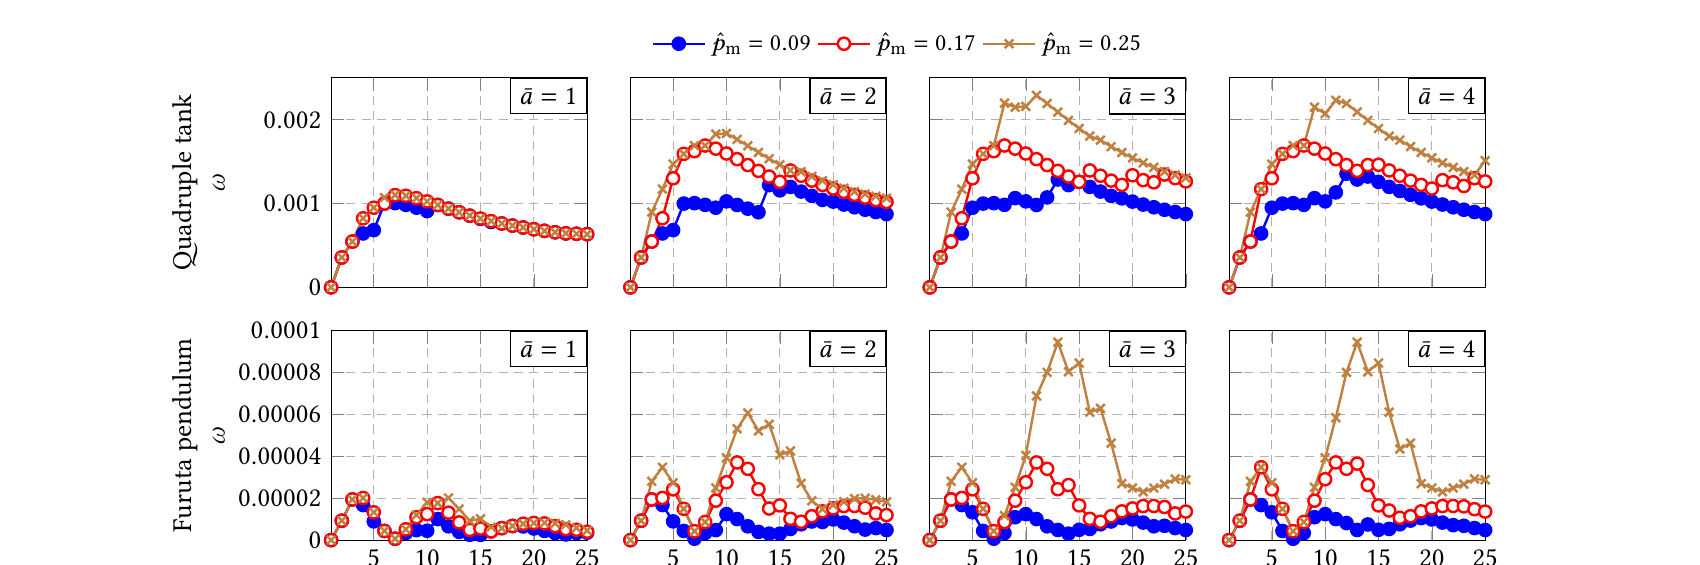
\includegraphics[width=.94\linewidth,height=3.8cm,keepaspectratio]{../assets/madhavi/fig2_paper.png}
\CPSCaption{Paper Fig.~2: tank HOLD (top), Furuta ZERO (bottom); columns $\bar a=1,\ldots,4$.}
\begin{block}{Takeaways}
\small\begin{itemize}\setlength\itemsep{1pt}
\item Effectiveness peaks around $\ell\approx10$--$13$, depending on the panel. Longer attacks are not always worse.
\item From $\bar a\approx3$, additional allowed consecutive misses barely change these curves.
\item Tank $\sim10^{-3}$ and Furuta $\sim10^{-5}$ use different output costs. Compare shapes only.
\end{itemize}
\end{block}
\src[Fig.~2]
\note{The x-axis is the attack horizon (1--25); each column fixes a watchdog cap. The curves vary the nominal miss scenario. The defender-side question motivates a study of configuration choices; the figure does not establish a universal watchdog threshold or a safety guarantee.}
\end{frame}

% ---------- 6. FIGURE 3 ----------
\begin{frame}{Figure 3: detector comparison}{Binomial, combined and geometric ($\chi^2$) tests; $\bar a=4$, $n_w=20$}
\gdef\CPSSourceContext{}
\gdef\CPSOrigin{PAPER}
\begin{columns}[T,onlytextwidth]
\begin{column}{.38\textwidth}
\centering
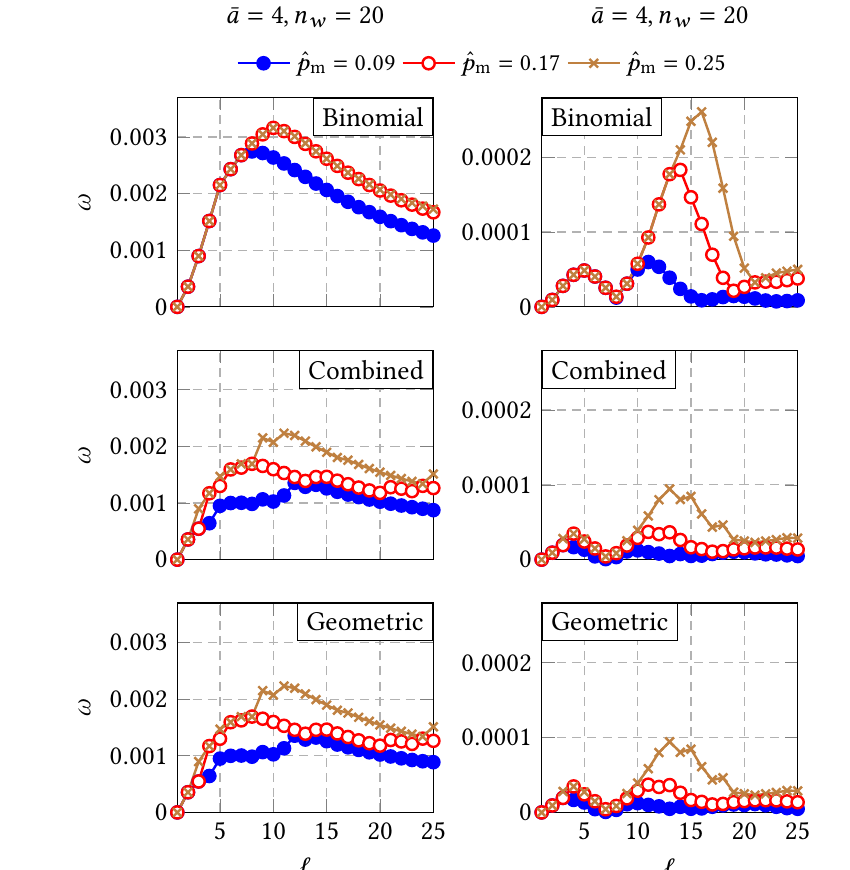
\includegraphics[width=\linewidth,height=5.6cm,keepaspectratio]{../assets/madhavi/fig3_paper.png}
\CPSCaption{Paper Fig.~3: tank HOLD (left), Furuta ZERO (right).}
\end{column}
\begin{column}{.60\textwidth}
\begin{block}{Takeaways}
\small\begin{itemize}\setlength\itemsep{.5em}
\item Rows compare binomial, combined and geometric ($\chi^2$) tests. The horizontal axis is $\ell$; curves use $\hat p_m=0.09,0.17,0.25$.
\item In these panels the combined and geometric ($\chi^2$) results coincide: the geometric ($\chi^2$) constraint is binding.
\item Our planned defender study includes all three detector choices. A fair ranking also needs an empirical session false-alarm comparison.
\end{itemize}
\end{block}
\end{column}
\end{columns}
\src[Fig.~3]
\note{The plotted configurations show a smaller feasible attack cost with the geometric ($\chi^2$) constraint. This is not a universal dominance theorem across plants, horizons or equal session false-alarm budgets. Multiple simultaneous windows remain a possible extension, not a completed result.}
\end{frame}

% ---------- 7. FIGURE 4 ----------
\begin{frame}{Figure 4: ZERO vs HOLD (Furuta)}{Window $n_w=10,12,\ldots,18$; $\bar a=4$; binomial test}
\gdef\CPSSourceContext{}
\gdef\CPSOrigin{PAPER}
\centering
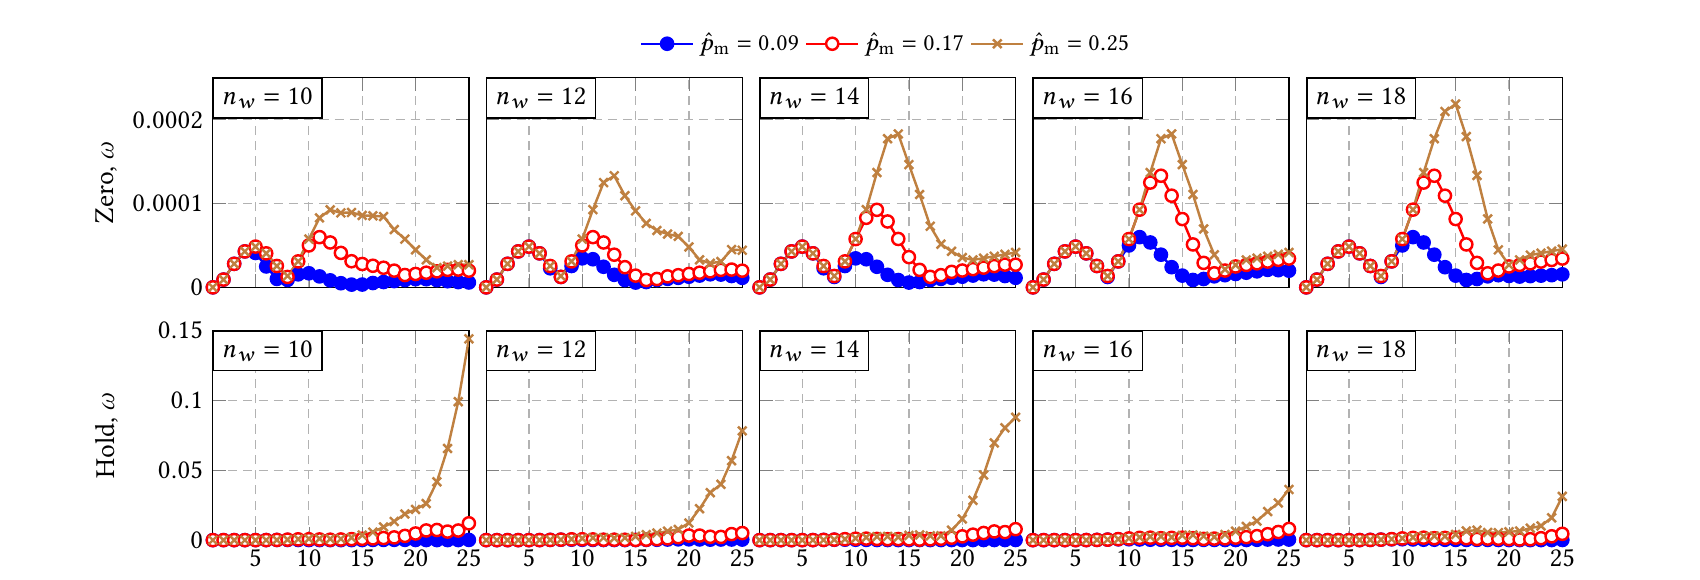
\includegraphics[width=.94\linewidth,height=3.7cm,keepaspectratio]{../assets/madhavi/fig4_paper.png}
\CPSCaption{Paper Fig.~4: ZERO (top) and HOLD (bottom); note the different vertical scales.}
\begin{block}{Takeaways}
\small\begin{itemize}\setlength\itemsep{1pt}
\item ZERO reaches about $2\times10^{-4}$; HOLD reaches about $0.15$ on this Furuta model.
\item Late bursts can strongly disrupt HOLD. ZERO keeps the terminal cost small on this plant.
\item Window length changes the attack budget and its timing. Policy selection requires plant-specific worst-case and false-alarm checks.
\end{itemize}
\end{block}
\src[Fig.~4]
\note{The original extension hook is a proposed defender-side policy and threshold sweep, not a demonstrated safe configuration. The later tank comparison explains why a ZERO rule cannot be transferred universally.}
\end{frame}

% ---------- 8. TABLE 1 ----------
\begin{frame}{Table 1: optimised attack sequences}{Furuta HOLD; $\hat p_m=.25$, $\bar a=4$, $\ell=25$; binomial test}
\gdef\CPSSourceContext{}
\gdef\CPSOrigin{PAPER}
\centering
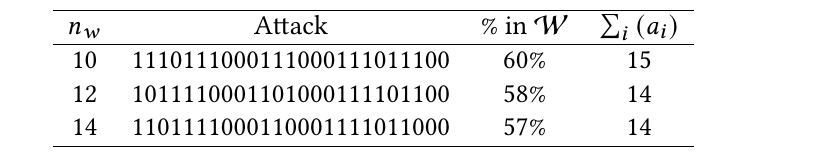
\includegraphics[width=.70\linewidth,height=2.3cm,keepaspectratio]{../assets/madhavi/table1_paper.png}
\CPSCaption{Paper Table~1: optimal miss schedules for three binomial-window lengths.}
\begin{block}{Takeaways}
\small\begin{itemize}\setlength\itemsep{.4em}
\item Each row reports the schedule, critical miss fraction in one window ($\%$ in $\mathcal W$), and total misses $\sum_i a_i$.
\item The fraction is the critical count divided by $n_w$: $6/10=60\%$, $7/12\approx58\%$, $8/14\approx57\%$.
\item \textbf{Link to our extension:} these attacks optimise against a fixed defence. We study how the defence configuration changes their worst-case cost.
\end{itemize}
\end{block}
\src[Table~1]
\note{The fraction in one window is different from the total number of misses over the 25-period horizon. All three sequences pass their binomial and watchdog checks; our later audit shows that they fail the geometric chi-square test. A wider window does not imply a monotone worst-case cost.}
\end{frame}

% ---------- 9. KEY FINDINGS ----------
\begin{frame}{Section 5: key findings}{Four results from the experiments}
\gdef\CPSSourceContext{}
\gdef\CPSOrigin{PAPER}
  \begin{columns}[T]
    \begin{column}{0.48\textwidth}
      \begin{block}{\textcolor{white}{(i) Impact isn't monotonic in $\ell$}}
        $\omega$ peaks around $\ell \approx 10$--$13$, depending on the panel; the optimiser concentrates or interleaves delays by initial conditions and budget.
      \end{block}
      \begin{block}{\textcolor{white}{(ii) Tight watchdogs help; loose ones add little}}
        In Fig.~2, $\bar a=1$--$2$ constrains the impact; from $\bar a=3$ the curves barely change.
      \end{block}
    \end{column}
    \begin{column}{0.48\textwidth}
      \begin{block}{\textcolor{white}{(iii) Geometric ($\chi^2$) constraint binds}}
        The geometric ($\chi^2$) and combined panels coincide in Fig.~3. Compare detectors under equal session false-alarm budgets before ranking them.
      \end{block}
      \begin{block}{\textcolor{white}{(iv) ZERO beats HOLD on the Furuta}}
        For the Furuta pendulum, zeroing the input on a miss is a far better defence; window length trades off per policy.
      \end{block}
    \end{column}
  \end{columns}
\end{frame}

% ---------- RESULTS -> EXTENSION ----------
\begin{frame}{From the paper's gaps to our extension}
\gdef\CPSSourceContext{}
\gdef\CPSOrigin{PAPER / OURS}
\begin{columns}[T,onlytextwidth]
\begin{column}{.47\textwidth}
\begin{block}{What the paper shows}
\small\begin{itemize}\setlength\itemsep{.6em}
\item Tight watchdogs ($\bar a\le2$) cut the impact; beyond $\bar a\approx3$ the curves are flat (Fig.~2).
\item A binding geometric ($\chi^2$) constraint in Fig.~3.
\item Strong policy sensitivity on Furuta in Fig.~4.
\item Attack optimisation against a \textbf{fixed} defence in Table~1.
\end{itemize}
\end{block}
\end{column}
\begin{column}{.51\textwidth}
\begin{block}{What we add}
\small\begin{itemize}\setlength\itemsep{.6em}
\item Defender formulation: minimise $\max_{\ell}\omega^*$ subject to a session false-alarm limit.
\item \textbf{Done:} independent reproduction, Furuta/tank policy replays, partial binomial sweep.
\item \textbf{Planned:} geometric ($\chi^2$) and combined-detector sweeps; missing $\ell=25$ solves; empirical false-alarm estimates.
\end{itemize}
\end{block}
\end{column}
\end{columns}
\medskip\small The paper asks how damaging an accepted attack can be. Our defender study asks which \emph{tested} configuration lowers that cost at an acceptable false-alarm rate.
\note{The dashboard shown later is a screenshot of an offline demonstration. A live demo, multiple simultaneous windows and a completed ranking are potential extensions, not delivered results. Preserve this distinction in the spoken hand-off.}
\end{frame}


\endgroup

% ==================== ABHISHEK (6 frames: speaker title + 5 original frames)
\begingroup
\makeatletter
\newcommand{\CPSAbhiAbar}{\ensuremath{\bar a}}
\newcommand{\CPSAbhiPhatm}{\ensuremath{\hat p_{\mathrm m}}}
\newcommand{\CPSAbhiTakeaway}[1]{{\small\color{black!80}#1\par}\vspace{1.2ex}}
\newcommand{\CPSAbhiCode}[1]{{\ttfamily #1}}

\tikzset{
  >={Latex[length=1.8mm]},
  arr/.style={->, thick, mgreenD},
  stage/.style={draw=mgreen, fill=mgreen, text=white, rounded corners=2pt, font=\scriptsize\bfseries,
                minimum height=0.62cm, text width=2.6cm, align=center},
  detail/.style={draw=rulec, fill=mgreenXL, rounded corners=2pt, font=\tiny, text width=2.6cm,
                 align=left, inner sep=1.5mm},
  box/.style={draw=mgreen, thick, fill=mgreenXL, rounded corners=2pt, font=\scriptsize, align=left, inner sep=1.6mm},
  darkbox/.style={draw=mgreenD, fill=mgreenD, text=white, rounded corners=2pt, font=\scriptsize, align=left, inner sep=1.6mm},
  dec/.style={diamond, aspect=1.9, draw=mgreen, thick, fill=mgreenL, font=\tiny, align=center, inner sep=0.4mm},
  reject/.style={draw=accent, fill=accentL, rounded corners=2pt, font=\tiny, align=center, inner sep=1.2mm, text width=2.3cm},
  pill/.style={draw=mgreen, fill=mgreenL, rounded corners=6pt, font=\tiny\bfseries, inner sep=1.4mm, align=center},
}

\def\CPSfootnote{}
\CPSUniformStyle

\colorlet{mgreen}{CPSgreen}
\colorlet{mgreenD}{CPSgreen!75!black}
\colorlet{mgreenM}{CPSgreen!65!white}
\colorlet{mgreenL}{CPSgreen!10}
\colorlet{mgreenXL}{CPSgreen!4}
\definecolor{accent}{HTML}{B4521C}
\definecolor{accentL}{HTML}{F8E6DA}
\colorlet{rulec}{CPSgreen!25!black!20}
% Retain readable diagram/detail sizes from the updated source.
\setbeamerfont{block body}{size=\scriptsize}
\setbeamerfont{block body alerted}{size=\scriptsize}
\beamer@calculateheadfoot
\makeatother

% ---------- SPEAKER TITLE ----------
\begin{frame}[c]
\gdef\CPSSourceContext{}
\gdef\CPSOrigin{OURS}
\CPSSpeakerTitleContent{4}{Setup \& Reproduction}
  {Paper Sections 3--5 and Appendix A.4.1}
  {The authors' code, all related cases and reproduction of the reduced experiment}
  {Abhishek Sharma}
\end{frame}

\begin{frame}{How the authors organised the code}{Driver, solver, saved results and plots}
\gdef\CPSSourceContext{}
\gdef\CPSOrigin{PAPER / OURS}
\small A driver selects one configuration. The detector-specific solver searches for its worst accepted attack, then the plotting files read the saved costs.
\vspace{.8em}
\begin{center}
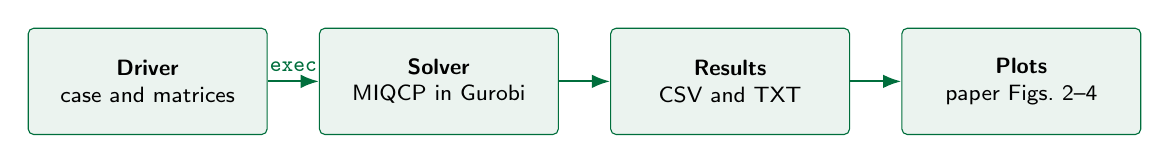
\begin{tikzpicture}[node distance=.65cm,
 p/.style={draw=CPSgreen,fill=CPSgreen!8,rounded corners=2pt,font=\footnotesize,align=center,text width=2.8cm,minimum height=1.35cm},
 a/.style={-{Latex},thick,CPSgreen}]
\node[p] (a) {\textbf{Driver}\\case and matrices};
\node[p,right=of a] (b) {\textbf{Solver}\\MIQCP in Gurobi};
\node[p,right=of b] (c) {\textbf{Results}\\CSV and TXT};
\node[p,right=of c] (d) {\textbf{Plots}\\paper Figs.~2--4};
\draw[a] (a)--node[above,font=\footnotesize]{\texttt{exec}}(b);
\draw[a] (b)--(c);\draw[a] (c)--(d);
\end{tikzpicture}
\CPSCaption{The authors' REP pipeline: one optimisation for each selected configuration and horizon.}
\end{center}
\begin{columns}[T,onlytextwidth]
\begin{column}{.49\textwidth}
\begin{block}{Drivers and model}
\footnotesize\texttt{main.py}, \texttt{main\_short.py}, \texttt{main\_fig2/3/4.py}.\par\medskip
\texttt{define\_system()} stores the closed-loop matrices; nested loops set the cases (paper Sections~3 and 5.1).
\end{block}
\begin{block}{How settings reach the solver}
\footnotesize\texttt{exec()} passes the loop settings as globals. Each figure driver changes the selected loop values.
\end{block}
\end{column}
\begin{column}{.49\textwidth}
\begin{block}{Three solver scripts}
\footnotesize\texttt{optimise\_bin.py}\\\texttt{optimise\_chi2.py}\\\texttt{optimise\_bin\_chi2.py}.\par\medskip
The combined script applies both statistical tests (paper Section~4, Eqs.~4--11).
\end{block}
\begin{block}{Result and plot files}
\footnotesize\texttt{results\_\{test\}/\{system\}/}; filenames encode $\bar a,\hat p_m,\alpha,n_w$. One row per saved length; TXT also stores schedules. \texttt{plot*.tex}, \texttt{fig/*.tex} and \texttt{Makefile} plot $\omega$ against $\ell$.
\end{block}
\end{column}
\end{columns}
\src[Authors' REP code; our code-structure explanation]

\note{The package is a flat pipeline of four layers, read left to right. Drivers: main.py runs everything, main\_short.py is a quick reduced run, main\_fig2, 3 and 4 each regenerate one figure. All share define\_system, which holds the hard-coded closed-loop matrices for each plant, and nested loops that pick each case (paper Sections 3 and 5.1). For every case the driver calls the solver with exec, so the loop variables reach it as globals. Solvers: one script per detector, binomial only, chi-square only, or both; each builds one mixed-integer optimisation and solves it with Gurobi (Section 4, Eqs 4 to 11). Results: every case appends rows to a CSV and a TXT whose folder and file name encode the case, one row per attack length. Plots: pgfplots files read the CSVs and draw Figures 2 to 4 (Section 5.4). Design choices at the bottom: one driver per figure, one solver per detector with the combined one a superset, exec instead of functions, and file names that encode the configuration.}
\end{frame}

\begin{frame}{Every case the code can run, and our focus}{Three plant setups and three detector choices}
\gdef\CPSSourceContext{}
\gdef\CPSOrigin{PAPER / OURS}
\footnotesize\renewcommand{\arraystretch}{1.35}
\begin{tabularx}{\linewidth}{>{\raggedright\arraybackslash}p{4.6cm}XXX}
\rowcolor{CPSgreen}\color{white}\textbf{Plant setup} & \color{white}\textbf{Binomial} & \color{white}\textbf{Geometric ($\chi^2$)} & \color{white}\textbf{Combined}\\
\rowcolor{CPSgreen!8}\texttt{furuta\_zero}: unstable; ZERO & Figs.~3, 4 & Fig.~3 & Figs.~2, 3; \textbf{our focus}\\
\texttt{furuta\_hold}: unstable; HOLD & Fig.~4, Table~1 & \texttt{main.py} & \texttt{main.py}\\
\rowcolor{CPSgreen!8}\texttt{qt\_nmp}: stable; HOLD & Fig.~3 & Fig.~3 & Figs.~2, 3\\
\end{tabularx}
\medskip
\begin{columns}[T,onlytextwidth]
\begin{column}{.55\textwidth}
\begin{block}{Driver to output}
\footnotesize\renewcommand{\arraystretch}{1.3}
\begin{tabularx}{\linewidth}{@{}lX@{}}
\texttt{main.py} & all 9 cases; full sweep\\
\texttt{main\_fig2.py} & Fig.~2; $\bar a=1$--$4$, $n_w=20$\\
\texttt{main\_fig3.py} & Fig.~3; $\bar a=4$, $n_w=20$\\
\texttt{main\_fig4.py} & Fig.~4/Table~1; $\bar a=4$, $n_w=10$--$18$\\
\texttt{main\_short.py} & one Fig.~2 curve; $\bar a=3$, $\hat p_m=.25$, $n_w=20$
\end{tabularx}
\end{block}
\end{column}
\begin{column}{.43\textwidth}
\begin{block}{Sweep and code conventions}
\footnotesize $\ell=1$--$25$, $\bar a=1$--$5$, $\hat p_m=.01,.03,\ldots,.25$, $n_w=10,12,\ldots,20$, $\alpha=.01$. Figure curves use $.09,.17,.25$.\par\medskip
Window longer than sequence: one binomial check. Geometric-only has no window: run once at 20. Boundary slots are hits. Tank output is half its level: output cost is REP cost divided by four.
\end{block}
\end{column}
\end{columns}
\begin{block}{Our focus: the reduced case}
\footnotesize \textbf{27 loop iterations}: \texttt{a\_length=1..27}; the intended plotted range has \textbf{25 positive-horizon rows}, $\ell=\texttt{a\_length}-2=1..25$. The authors estimate about 2 h for this reduced experiment; the full driver has 68,445 calls. Our independent enumeration uses the \textbf{same model and constraints}, rather than re-running Gurobi.
\end{block}
\src[REP drivers; Appendix A.4.1]

\note{A case is a plant configuration times a detector. The pendulum is open-loop unstable and was also run on real hardware; it appears with the zero policy (motor gets zero on a missed deadline) and the hold policy (keeps its last value). The quadruple tank is open-loop stable and non-minimum phase and uses hold. Detectors: binomial only, chi-square only, or both; the watchdog is always on. That gives nine cases; each cell says which figure or table uses it; hold with chi-square and hold with both are computed only by main.py. The diagram shows which driver produces which output and what it fixes: main.py sweeps everything, main\_fig2 fixes window 20 and varies the watchdog limit 1 to 4, main\_fig3 fixes a-bar 4 and window 20 to compare detectors, main\_fig4 fixes a-bar 4 and varies the window 10 to 18, and main\_short fixes one case. Special cases: window longer than the attack gives a single binomial constraint; chi-square only ignores the window so it runs once at 20; first and last slots are forced hits so 27 slots give lengths 1 to 25; the tank's output is half its level so plots divide omega by 4. Our focus is the highlighted cell: 27 loop iterations rather than 68,445 driver calls, with 25 intended positive-horizon plotted rows; the authors estimate about 2 hours for the reduced case, while our enumeration uses the same model and constraints; the authors use it as their environment test (Appendix A.4.1).}
\end{frame}

\begin{frame}{How main\_short.py runs, step by step}{Part 4 \textperiodcentered{} the code}
\gdef\CPSSourceContext{}
\gdef\CPSOrigin{PAPER / OURS}
\note{Left: main\_short.py sets alpha 0.01, loads the pendulum with the zero policy from define\_system (the 7 by 7 matrices Phi-h and Phi-m, Q on the angle, the start state), creates the results folder (if it exists it prints already done and carries on, unlike main.py which exits), then loops a\_length from 1 to 27 and runs optimise\_bin\_chi2.py with exec each time. Right: nine steps; steps 5 to 9 are the paper's equations. Step 3: zs are the attack bits, xs the closed-loop states psi = [x; y-tilde; z; u], 3 + 3 + 0 + 1 = 7 numbers, bounded to plus or minus 1000 or Gurobi calls the model unbounded. Step 4: first and last slots are forced hits, so every run of misses is closed by a hit; that is why 27 slots give lengths 1 to 25. Step 5: indicator constraints, z = 0 enforces the hit equation, z = 1 the miss equation; for the zero policy the last row of Phi-miss is zero. Step 6: any 4 slots hold at most 3 misses. Step 7: binom.ppf(0.99, 20, 0.25) = 10. Step 8, the chi-square trick: aux = (1 - z\_i) + the k middle bits + (1 - z\_(i+k+1)) - (k+1) equals 1 only for hit, k misses, hit; max(aux, 0) counts runs m\_k; N = sum of m\_k; expected p\_k N with p\_k = 0.75, 0.19, 0.05, 0.02; since N is a variable the critical value 11.34 is multiplied by N instead of dividing. Step 9: maximise xs[L-1]' Q xs[L-1] and append the best row.}
\CPSAbhiTakeaway{The author driver loops over 27 values of \texttt{a\_length}. Its plotted positive horizons are $\ell=1,\ldots,25$.}

\begin{center}
\begin{tikzpicture}[
  fbox/.style={box, text width=4.1cm, minimum height=0.8cm},
]
\node[font=\scriptsize\bfseries, text=mgreen, anchor=west] at (0,0.35) {MAIN\_SHORT.PY \textperiodcentered{} DRIVER};
\node[fbox, anchor=north west] (a) at (0,0) {Start: load the pendulum (zero policy)\\ {\color{mgreen}\ttfamily define\_system('furuta\_zero')}};
\node[fbox, below=0.22cm of a] (b) {Make the results folder\\ {\color{body}already there $\to$ warns, carries on}};
\node[dec, aspect=2.4, font=\scriptsize, below=0.22cm of b] (d) {\textbf{more lengths?}\\a\_length 1 \dots{} 27};
\node[darkbox, text width=4.1cm, minimum height=0.8cm, below=0.4cm of d] (e) {\textbf{Target: 25 plotted rows}\\ plot\_short.tex $\to$ $\omega$ vs $\ell$ plot};
\draw[arr] (a) -- (b);
\draw[arr] (b) -- (d);
\draw[arr] (d) -- node[right, font=\scriptsize]{\bfseries no} (e);

\node[font=\scriptsize\bfseries, text=mgreenD, anchor=west] at (6.0,0.35) {OPTIMISE\_BIN\_CHI2.PY \textperiodcentered{} SOLVER, ONCE PER $\ell$};
\node[draw=mgreenD, thick, fill=mgreenXL, rounded corners=2pt, anchor=north west, inner sep=1.8mm, font=\scriptsize] (s) at (6.0,0) {\parbox[t][3.55cm][t]{8.1cm}{%
\renewcommand{\arraystretch}{1.12}%
\begin{tabular}{@{}>{\color{mgreen}\bfseries\ttfamily}l@{\hspace{2mm}}l@{}}
1 & Open the output files (CSV and TXT, append)\\
2 & Set up Gurobi: silent, keep 3 solutions, tolerance 1e-9\\
3 & Unknowns: attack bits zs $=a_i$, states xs $=\psi$ ($\pm$1000)\\
4 & First and last slot forced on time (zs $=0$)\\
5 & \textbf{Eq.~4} next state: on time $\Rightarrow\Phi_h$, late $\Rightarrow\Phi_m$ (indicator \texttt{>>})\\
6 & \textbf{Eq.~7 constraint} watchdog: at most 3 misses in any 4 slots\\
7 & \textbf{Eq.~9} binomial: at most 10 misses per 20 slots\\
8 & \textbf{Eqs 10--11} $T=N S_{\chi^2}\le11.345\,N$\\
9 & \textbf{Goal}: largest pendulum angle$^2$ at the end $\to$ save row\\
\end{tabular}}};
\draw[arr, mgreen] (d.east) -- node[above, font=\scriptsize]{\bfseries yes} ($(d.east -| s.west)+(-0.75,0)$) |- ($(s.north west)+(0,-0.42)$);
\draw[arr, accent] (d.south east -| s.west) -- node[below, font=\scriptsize]{\bfseries next $\ell$} (d.south east);
\node[anchor=north west, text width=8.1cm, font=\tiny, text=body, align=left] at ($(s.south west)+(0,-0.12)$) {\texttt{exec()} hands over a\_length, $\bar a=3$, $\hat p_{\mathrm m}=0.25$, $n_w=20$, $\Phi_h$, $\Phi_m$ as globals. Output: \texttt{a3\_p0.25\_alpha0.01\_w20.csv / .txt}};
\end{tikzpicture}
\end{center}
\CPSCaption{Author-driver control flow; output requires a successful solve, not merely a loop iteration.}

\note{The two values a_length=1,2 do not represent positive attack horizons. The driver catches exceptions; saved rows depend on feasibility, status and licence. It is inaccurate to equate 27 loop iterations with 27 successful positive-horizon solves. The independent curve on the next result slide was obtained by enumeration, not by these Gurobi calls.}
\end{frame}

\begin{frame}{Worked example: how the model selects an attack}{Part 4 \textperiodcentered{} the code}
\gdef\CPSSourceContext{}
\gdef\CPSOrigin{OURS}
\note{The stored sequence length is ell+2=7; the five interior bits give 32 candidates. The initial angle is 0.0097627 rad. The watchdog removes 0111100 because it contains four consecutive misses. The binomial allowance is 10 misses per 20-slot window and cannot bind with five free bits. For the geometric (chi-square) test use the textbook statistic S: 0111000 has S=20.111, 0101010 has S=13.0 and 0110100 has S=6.333. All three have N=3 counted hit-to-hit intervals; the df=3 critical value is 11.344867 at alpha=.01. The REP numerator is T=N*S, giving 60.333,39,19 with scaled limit 34.0346. The winning interior sequence 11010 matches paper Section 5.4.1. The replay ends near .00603 rad under attack versus .00299 nominal, giving terminal costs 3.63 and .89 times 1e-5 and omega about 2.74e-5. These are model-based finite-horizon costs, not a physical failure certificate.}
\CPSAbhiTakeaway{$\ell=5$ (stored length $\ell+2=7$): 32 possible attacks. Three checks remove the risky ones; the most damaging survivor wins.}

\begin{center}
\begin{tikzpicture}[node distance=0.2cm]% PATCH: was 0.3cm, diagram was wider than the text block
\node[box, text width=1.6cm, align=center, font=\tiny] (st) {\textbf{32 attacks}\\$z_1\dots z_5$ free\\(ends forced on time)};
\node[dec, right=of st, text width=1.2cm] (w) {\textbf{Watchdog}\\$\le3$ in any\\4 slots?};
\node[dec, right=of w, text width=1.2cm] (bn) {\textbf{Binomial}\\$\le10$ per\\20 slots?};
\node[dec, right=of bn, text width=1.2cm] (cs) {\textbf{Geometric ($\chi^2$)}\\$S_{\chi^2}$\\$\le11.345$?};
\node[box, right=of cs, text width=1.6cm, align=center, font=\tiny] (mx) {\textbf{Maximise}\\angle$^2$ at step 6\\among survivors};
\node[darkbox, right=of mx, text width=1.75cm, align=center, font=\tiny] (wn) {\textbf{Winner}\\\texttt{0 11010 0}\\$\omega=2.74\times10^{-5}$};
\draw[arr] (st) -- (w);
\draw[arr] (w) -- node[above, font=\tiny]{yes} (bn);
\draw[arr] (bn) -- node[above, font=\tiny]{yes} (cs);
\draw[arr] (cs) -- node[above, font=\tiny]{yes} (mx);
\draw[arr] (mx) -- (wn);
\node[reject, below=0.3cm of w] (rw) {\textbf{reject} \texttt{0111100}\\4 in a row $\to$ shutdown};
\node[reject, below=0.3cm of bn, draw=rulec, fill=mgreenXL] (rb) {cannot bind here\\(only 5 free slots)};
\node[reject, below=0.3cm of cs] (rc) {\textbf{reject} \texttt{0111000} ($S=20.1$)\\and \texttt{0101010} ($S=13.0$)};
\draw[arr, accent] (w) -- node[right, font=\tiny]{no} (rw);
\draw[arr, body!60] (bn) -- (rb);
\draw[arr, accent] (cs) -- node[right, font=\tiny]{no} (rc);
\end{tikzpicture}
\end{center}
{\footnotesize $S_{\chi^2}=\sum_r(m_r-p_rN)^2/(p_rN)$. REP uses $T=N S_{\chi^2}$.
For the winner, $N=3$: $T=19.0\le11.345\times3\approx34.0$ ($\bar a=3$, $\alpha=.01$).\par}
\vspace{0ex}

\begin{columns}[T,onlytextwidth]
\begin{column}{0.5\textwidth}
{\scriptsize
\renewcommand{\arraystretch}{1.02}\setlength{\tabcolsep}{4pt}
\noindent\begin{tabular}{l l r l}
\rowcolor{mgreen}\color{white}\textbf{Attack} & \color{white}\textbf{Check} & \color{white}\textbf{angle$^2$} & \color{white}\textbf{Result}\\
\rowcolor{mgreenXL}\ttfamily 0000000 & no attack & 0.89 & baseline\\
\rowcolor{mgreenL}\ttfamily 0111100 & 4 in a row & 5.75 & watchdog stop\\
\rowcolor{mgreenXL}\ttfamily 0111000 & $S=20.1>11.345$ & 4.99 & burst too rare\\
\rowcolor{mgreenL}\ttfamily 0101010 & $S=13.0>11.345$ & 2.22 & too regular\\
\rowcolor{accentL}\ttfamily\bfseries 0110100 & \textbf{$S=6.33\le11.345$} & \textbf{3.63} & \textbf{chosen: hidden}\\
\end{tabular}\\[0.3ex]
{\tiny\color{body} angle$^2$ at step 6, in units of $10^{-5}$}}
\end{column}
\begin{column}{0.47\textwidth}
\begin{tikzpicture}
\begin{axis}[
  width=\linewidth, height=2.5cm,% PATCH: was 3.3cm
  xmin=0, xmax=6, ymin=0.0025, ymax=0.0105,
  xtick={0,...,6}, ytick={0.003,0.006,0.009},
  yticklabel style={/pgf/number format/fixed,/pgf/number format/precision=3},
  scaled y ticks=false,
  xlabel={step $k$}, ylabel={angle (rad)}, xlabel style={yshift=0.8ex},
  label style={font=\tiny}, tick label style={font=\tiny},
  legend style={font=\tiny, draw=none, fill=none, at={(0.5,-0.55)}, anchor=north}, legend columns=2,
  grid=major, grid style={dashed, rulec},
  title={\scriptsize\bfseries\color{mgreen} Pendulum angle: winner vs no attack}, title style={yshift=-1.5ex},
]
\addplot[accent, thick, mark=*, mark size=1.2pt] coordinates {(0,0.00976)(1,0.01000)(2,0.00981)(3,0.00919)(4,0.00861)(5,0.00756)(6,0.00603)};
\addlegendentry{with attack \texttt{0110100}}
\addplot[mgreen, thick, mark=square*, mark size=1.1pt] coordinates {(0,0.00976)(1,0.01000)(2,0.00981)(3,0.00867)(4,0.00679)(5,0.00473)(6,0.00299)};
\addlegendentry{no attack}
\node[font=\tiny, anchor=west] at (axis cs:4.1,0.0067) {0.0060};
\node[font=\tiny, anchor=west] at (axis cs:5.05,0.0034) {0.0030};
\end{axis}
\end{tikzpicture}
\end{column}
\end{columns}
\CPSCaption{Candidate schedules and the same-initial-state angle replay; angle-squared costs use $10^{-5}$.}
\end{frame}

\begin{frame}{Independent reproduction of the Furuta curve}{Furuta, ZERO policy; combined tests; $\bar a=3$, $\hat p_m=.25$, $n_w=20$, $\alpha=.01$}
\gdef\CPSSourceContext{}
\gdef\CPSOrigin{OURS}
\begin{columns}[T,onlytextwidth]
\begin{column}{.54\textwidth}
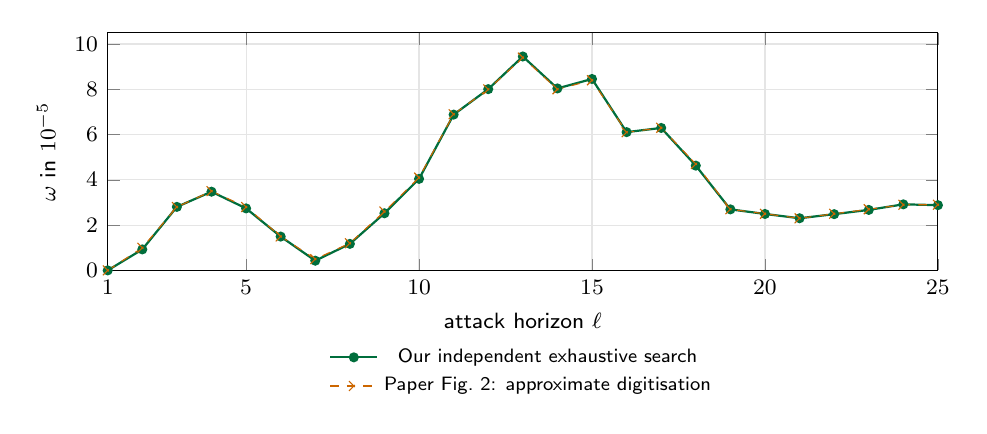
\begin{tikzpicture}
\begin{axis}[width=\linewidth,height=4.6cm,xmin=1,xmax=25,ymin=0,ymax=10.5,
xtick={1,5,10,15,20,25},ytick={0,2,4,6,8,10},xlabel={attack horizon $\ell$},ylabel={$\omega$ in $10^{-5}$},
label style={font=\footnotesize},tick label style={font=\footnotesize},grid=major,grid style={gray!20},
legend style={font=\scriptsize,draw=none,at={(.5,-.28)},anchor=north},legend columns=1]
\addplot[CPSgreen,thick,mark=*,mark size=1.4pt] table[x=ell,y=omega_e5,col sep=comma,row sep=\\]{
ell,omega_e5\\
1,0\\2,0.927\\3,2.806\\4,3.477\\5,2.739\\6,1.494\\7,0.428\\8,1.171\\9,2.523\\10,4.043\\11,6.882\\12,8.007\\13,9.45\\14,8.038\\15,8.456\\16,6.108\\17,6.293\\18,4.628\\19,2.696\\20,2.493\\21,2.303\\22,2.484\\23,2.672\\24,2.918\\25,2.882\\};
\addlegendentry{Our independent exhaustive search}
\addplot[orange!80!black,dashed,mark=x,mark size=2.5pt] coordinates {(1,0)(2,1.0)(3,2.8)(4,3.5)(5,2.8)(6,1.5)(7,.5)(8,1.2)(9,2.6)(10,4.1)(11,6.9)(12,8.0)(13,9.4)(14,8.0)(15,8.4)(16,6.1)(17,6.3)(18,4.7)(19,2.7)(20,2.5)(21,2.3)(22,2.5)(23,2.7)(24,2.9)(25,2.9)};
\addlegendentry{Paper Fig.~2: approximate digitisation}
\end{axis}
\end{tikzpicture}
\CPSCaption{Same axes; the paper series is a low-resolution graphical reference, not raw author data.}
\end{column}
\begin{column}{.44\textwidth}
\footnotesize\renewcommand{\arraystretch}{1.35}
\begin{tabularx}{\linewidth}{@{}Xcc@{}}
\toprule & \textbf{Ours} & \textbf{Paper plot}\\
\midrule Peak $\omega$ ($10^{-5}$) & 9.45 & $\approx9.4$\\
Peak at $\ell$ & 13 & $\approx13$\\
\bottomrule
\end{tabularx}
\begin{block}{Two checkable sequences}
\footnotesize $\ell=5$: \texttt{11010}\\[.5em]
$\ell=15$: \texttt{101011011101000}.\par\medskip
Our curve uses $\bar a=3$; the matching sequences quoted in paper Section~5.4.1 use $\bar a=4$. Neither needs more than three consecutive misses. The printed sequences omit REP's forced boundary hits.
\end{block}
\begin{block}{Method and interpretation}
\footnotesize Independent enumeration, about 6 min, with the authors' matrices and the same constraints. Short attacks exploit the initial tilt; the peak interleaves hits/misses; longer attacks wait and strike late.
\end{block}
\end{column}
\end{columns}
\vspace{.2em}\footnotesize The largest difference to the rounded graphical reference is below $0.08\times10^{-5}$; digitisation uncertainty is about $0.15\times10^{-5}$. This is visual agreement, not an exact raw-data error bound.
\src[Our enumeration; paper Fig.~2/Section~5.4.1; project links in glossary]

\note{This curve is an independent exhaustive enumeration with the official matrices, initial state, boundary hits, watchdog and statistical constraints; it is not a Gurobi rerun. The recorded project run took about six minutes. The 25 values are retained from omega_main_short.csv. Our peak is 9.45e-5 at ell=13. The overlaid paper reference is a rounded graphical reading of the supplied Fig. 2 panel, so its peak is approximately 9.4e-5 near 13; the apparent maximum difference below .08e-5 is smaller than the roughly .15e-5 digitisation uncertainty. It is not an exact comparison to the authors' raw CSVs. The paper explicitly prints 11010 at ell=5 and 101011011101000 at ell=15 for a-bar=4; the schedules also pass a-bar=3 because they never use a longer burst. Short attacks exploit the initial tilt, the peak interleaves misses and hits, and long attacks wait before striking late. The authors' main_short.py can append duplicate rows on rerun and catches failures with a bare except. A restricted Gurobi licence prevents some larger models.}
\end{frame}

\endgroup

% ==================== SRINJOY (7 frames: speaker title + 6 original frames)
\begingroup
\makeatletter




\pgfplotsset{compat=1.18}
\definecolor{forest}{HTML}{00704A}
\definecolor{deepgreen}{HTML}{00583B}
\definecolor{holdred}{HTML}{B42332}
\definecolor{zeroteal}{HTML}{087F8C}
\definecolor{ink}{HTML}{16372C}








\setlength{\parskip}{1mm}
\pgfplotsset{trace/.style={axis line style={gray!60},tick style={gray!60},
 grid=major,grid style={gray!15},tick label style={font=\scriptsize},
 label style={font=\scriptsize},every axis plot/.append style={line join=round},
 scaled x ticks=false,xticklabel style={/pgf/number format/fixed,/pgf/number format/precision=3},
 enlarge x limits=false}}
\newcommand{\source}[1]{\src[#1]}
\title{Visualisation Cases and Defender Extension}
\hypersetup{pdftitle={Stealthy Computational Delay Attacks on Control Systems},pdfsubject={Combined CS637 paper review, reproduction and defender study}}

\def\CPSfootnote{}
\CPSUniformStyle
\beamer@calculateheadfoot
\makeatother


% Slide 1: three Table 1 presets, all replayed through both policies.
% ---------- SPEAKER TITLE ----------
\begin{frame}[c]
\gdef\CPSSourceContext{}
\gdef\CPSOrigin{OURS}
\CPSSpeakerTitleContent{5}{Visualisation Cases and Defender Extension}
  {Paper Section 5: Experimental Results}
  {Results replay and validation \textperiodcentered{} Project extension: defender configuration}
  {Srinjoy Chakraborty}
\end{frame}

\begin{frame}[t,shrink=5]{Furuta: the three published HOLD attacks}
\gdef\CPSSourceContext{}
\gdef\CPSOrigin{OURS}
\small
\(\ell=25,\ \hat p_m=0.25,\ \bar a=4,\ \alpha=0.01,\ T_s=5\,\mathrm{ms}\).
The same schedule and initial state drive both policies.
\vspace{1mm}
\begin{columns}[T,onlytextwidth]
\column{0.51\textwidth}
\begin{tikzpicture}
\begin{axis}[trace,width=\linewidth,height=3.0cm,% PATCH: was 3.65cm
 xlabel={Time after initial forced hit (s)},ylabel={Pendulum angle (deg)},
 xmin=0,xmax=.125,ymin=-24,ymax=4,
 legend style={at={(.02,.03)},anchor=south west,font=\tiny,draw=none,fill=white},
 legend columns=2]
\addplot[holdred,thick,] coordinates {(0,0.5731552492) (0.005,0.562169538) (0.01,0.4985888844) (0.015,0.3820828321) (0.02,0.2120458485) (0.025,-0.01438817278) (0.03,-0.3003784578) (0.035,-0.6474114227) (0.04,-1.057290749) (0.045,-1.460833361) (0.05,-1.671777621) (0.055,-1.579928442) (0.06,-1.190562619) (0.065,-0.5016564478) (0.07,0.4903706165) (0.075,1.712267672) (0.08,2.676624247) (0.085,2.88379653) (0.09,2.245559595) (0.095,0.7585962475) (0.1,-1.584821909) (0.105,-4.643739351) (0.11,-8.280919318) (0.115,-12.51526582) (0.12,-17.36878659) (0.125,-21.75198247)};\addlegendentry{HOLD, \(n_w=10\)}
\addplot[blue,thick,] coordinates {(0,0.5731552492) (0.005,0.562169538) (0.01,0.4985888844) (0.015,0.3801004821) (0.02,0.2041061453) (0.025,-0.03030884528) (0.03,-0.3243628463) (0.035,-0.6795841844) (0.04,-1.066461047) (0.045,-1.328987201) (0.05,-1.32653314) (0.055,-1.043751086) (0.06,-0.4791712967) (0.065,0.3098699196) (0.07,1.26720288) (0.075,2.130908973) (0.08,2.478988649) (0.085,2.222320762) (0.09,1.428235349) (0.095,0.09260520089) (0.1,-1.791511533) (0.105,-4.233907427) (0.11,-7.070905883) (0.115,-10.14088122) (0.12,-13.45978945) (0.125,-16.02556158)};\addlegendentry{HOLD, \(n_w=12\)}
\addplot[orange,thick,] coordinates {(0,0.5731552492) (0.005,0.562169538) (0.01,0.4985888844) (0.015,0.3820828321) (0.02,0.2100634985) (0.025,-0.02034552597) (0.03,-0.3103417771) (0.035,-0.6614324918) (0.04,-1.075442441) (0.045,-1.504341655) (0.05,-1.760111189) (0.055,-1.69676499) (0.06,-1.30672478) (0.065,-0.5879633506) (0.07,0.3855656261) (0.075,1.223912398) (0.08,1.528060639) (0.085,1.213537782) (0.09,0.2787091129) (0.095,-1.281284079) (0.1,-3.474549757) (0.105,-6.215733162) (0.11,-9.422327299) (0.115,-13.11099824) (0.12,-16.24281245) (0.125,-16.99621636)};\addlegendentry{HOLD, \(n_w=14\)}
\addplot[zeroteal,thick,dashed] coordinates {(0,0.5731552492) (0.005,0.562169538) (0.01,0.5263472755) (0.015,0.4932606689) (0.02,0.4627377527) (0.025,0.4048791449) (0.03,0.3193841292) (0.035,0.2355490918) (0.04,0.1529383055) (0.045,0.05563556085) (0.05,-0.04759294443) (0.055,-0.1204862538) (0.06,-0.1726951481) (0.065,-0.2258016142) (0.07,-0.2800816697) (0.075,-0.3160593638) (0.08,-0.3160900955) (0.085,-0.2912470148) (0.09,-0.2592325941) (0.095,-0.2285655182) (0.1,-0.1990863967) (0.105,-0.1712592288) (0.11,-0.1449393847) (0.115,-0.1193728536) (0.12,-0.09442675529) (0.125,-0.07702961586)};
\addlegendentry{ZERO, \(n_w=10\)}
\end{axis}
\end{tikzpicture}

\column{0.46\textwidth}
\centering
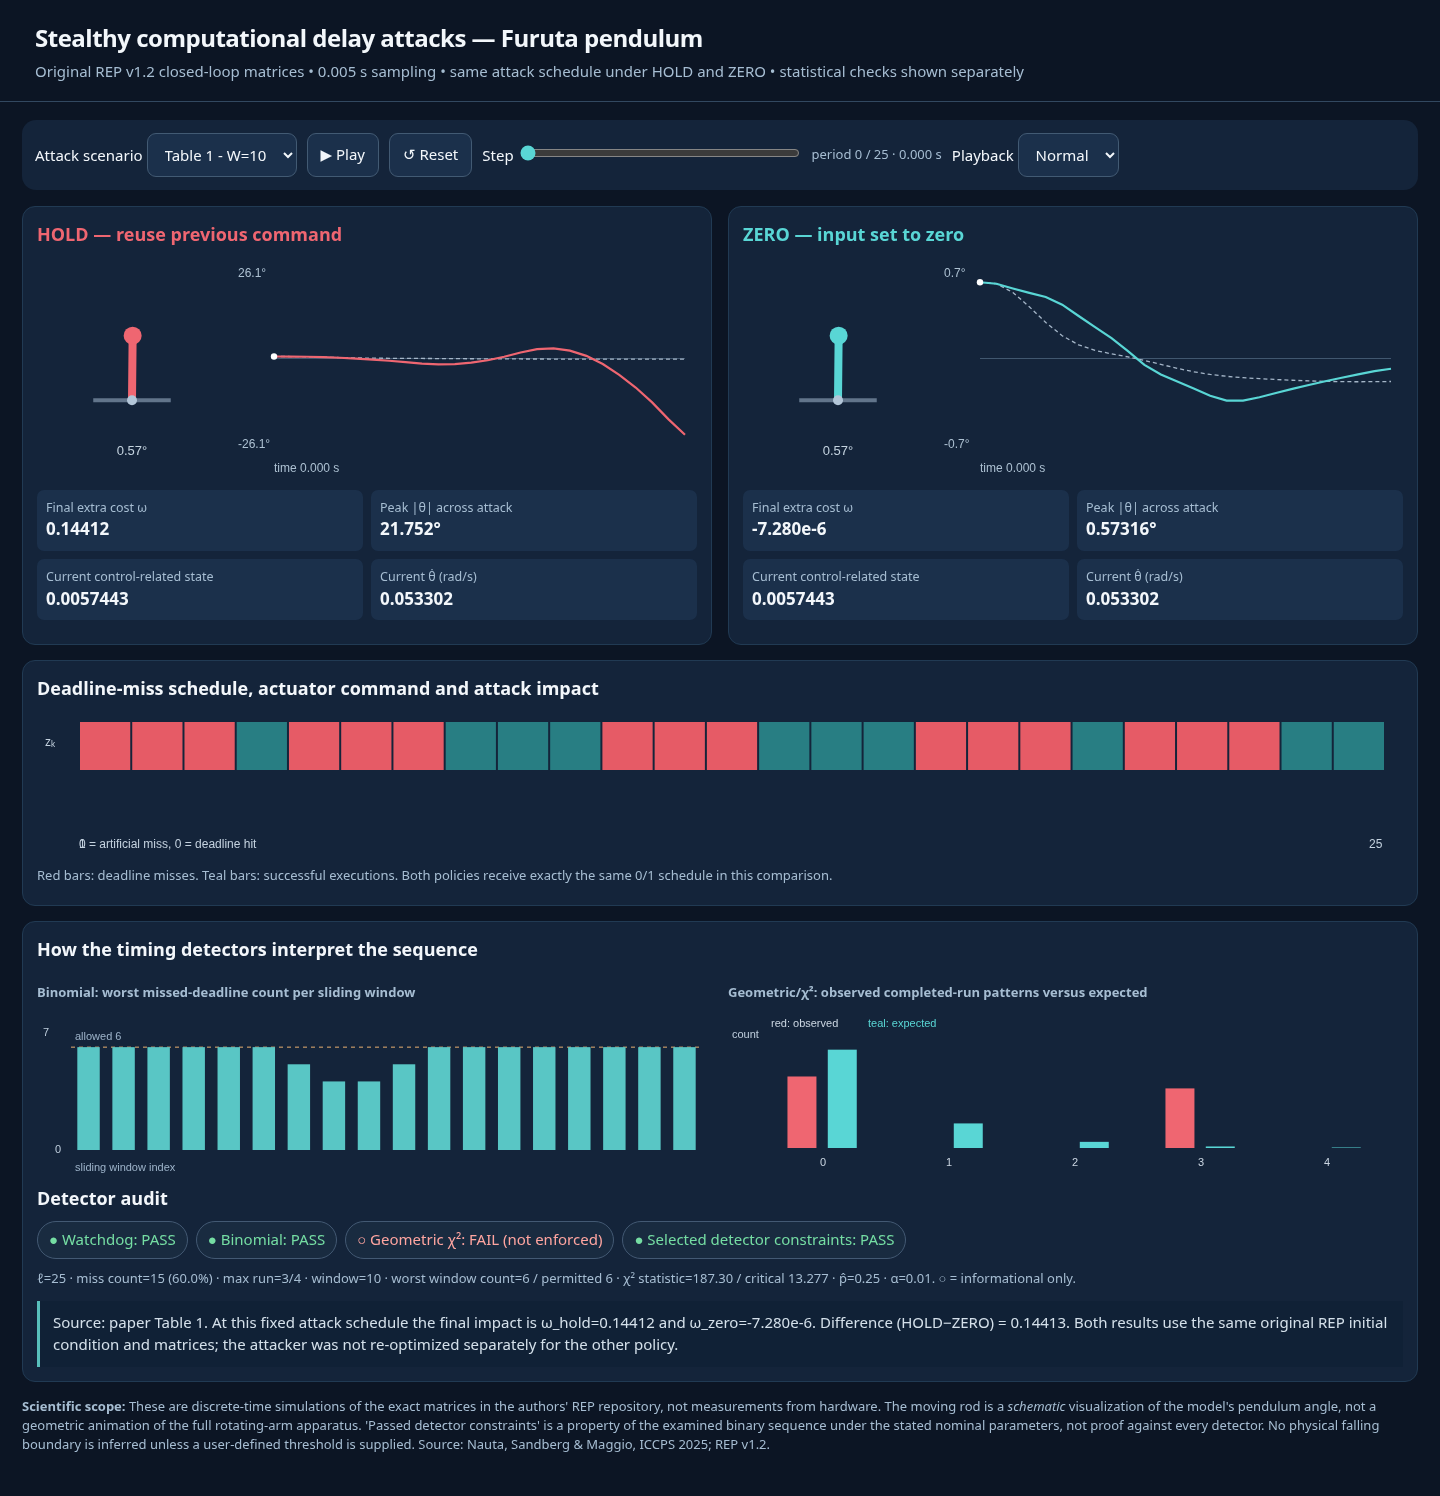
\includegraphics[trim=20bp 835bp 20bp 200bp,clip,width=\linewidth]{../assets/srinjoy/furuta_dashboard.png}
\vspace{1mm}
\raggedright\footnotesize
Offline dashboard screenshot: schematic angle view.
\par\vspace{2mm}
All pass watchdog and binomial. The geometric ($\chi^2$) test rejects all three:
\(S_{\chi^2}=187.30,\ 86.22,\ 94.78>13.277\).\par\vspace{1mm}{\scriptsize Textbook statistic; $\bar a=4$, $\alpha=.01$, critical value $\chi^2_{.99}(4)=13.277$.}
\end{columns}
\vspace{1mm}\par{\centering\scriptsize
\begin{tabular}{@{}ccrrr@{}}
\toprule
Window & Misses & \(\omega_{\rm HOLD}\) (rad\(^2\)) & \(\omega_{\rm ZERO}\), same attack & Peak \(|\theta|\), HOLD\\
\midrule
10 & 15 & 0.144120 & \(-7.28\!\times\!10^{-6}\) & 21.75$^\circ$ \\
12 & 14 & 0.078222 & \(-5.72\!\times\!10^{-6}\) & 16.03$^\circ$ \\
14 & 14 & 0.087986 & \(-7.36\!\times\!10^{-6}\) & 17.00$^\circ$ \\

\bottomrule
\end{tabular}\par}
\vspace{1mm}\raggedright
\footnotesize\textbf{Observation:} same-schedule replay supports the paper's actuation-policy sensitivity.
\CPSCaption{Our replay of paper Table~1 schedules: the attacks optimise HOLD under the binomial test.}
{\footnotesize $\omega<0$: the schedule leaves a smaller terminal cost than nominal under ZERO. This does not bound the ZERO worst case; the attacker must be re-optimised for ZERO.\par}
\src[Our replay of Table~1; project links in glossary]
\note{All three published sequences and their detector audits come from the project replay package.
The numerical routines in rep\_paper\_visuals.py were used unchanged. The zero-policy
curves use each HOLD-optimised sequence without re-optimising. Negative omega means
that this fixed schedule has a smaller terminal angle cost than nominal at the scored
sample. It does not bound the ZERO worst case. Physical time starts after the first
forced hit. All values score the state before the last forced hit.
Source paper: https://doi.org/10.1145/3716550.3722013 .}
\end{frame}


% Slide 2: all remaining Furuta presets in the additional project replay.
\begin{frame}[t]{Furuta: horizon and detector validation}
\gdef\CPSSourceContext{}
\gdef\CPSOrigin{OURS}
\small
The published ZERO cases use the combined detector with \(n_w=20\).
The extra 23-period replay uses binomial detection with \(n_w=10\).
\vspace{2mm}
\begin{columns}[T,onlytextwidth]
\column{0.49\textwidth}
\begin{tikzpicture}
\begin{axis}[trace,width=\linewidth,height=4.45cm,
 xlabel={Time after initial forced hit (s)},ylabel={ZERO angle (deg)},
 xmin=0,xmax=.125,
 legend style={at={(.98,.98)},anchor=north east,font=\scriptsize,draw=none,fill=white}]
\addplot[blue,thick,] coordinates {(0,0.5731552492) (0.005,0.562169538) (0.01,0.5263472755) (0.015,0.4932606689) (0.02,0.4329970116) (0.025,0.3452430871)};\addlegendentry{\(\ell=5\)}
\addplot[holdred,thick,] coordinates {(0,0.5731552492) (0.005,0.562169538) (0.01,0.5263472755) (0.015,0.4635199278) (0.02,0.3733609538) (0.025,0.269948985) (0.03,0.1527465442) (0.035,0.03633799374) (0.04,-0.07504831727) (0.045,-0.1819913119) (0.05,-0.2898801947) (0.055,-0.399275711) (0.06,-0.486759363) (0.065,-0.5527858414) (0.07,-0.5828105344) (0.075,-0.5436788959)};\addlegendentry{\(\ell=15\)}
\addplot[zeroteal,thick,] coordinates {(0,0.5731552492) (0.005,0.562169538) (0.01,0.5263472755) (0.015,0.4932606689) (0.02,0.4329970116) (0.025,0.3299074915) (0.03,0.2157215646) (0.035,0.1191409503) (0.04,0.05307100042) (0.045,0.0142560929) (0.05,-0.009283260466) (0.055,-0.02952695976) (0.06,-0.05306166571) (0.065,-0.07919951235) (0.07,-0.1068343766) (0.075,-0.1361098889) (0.08,-0.1660928235) (0.085,-0.1946273069) (0.09,-0.2218616452) (0.095,-0.2502490951) (0.1,-0.2799371985) (0.105,-0.3040567942) (0.11,-0.3227332423) (0.115,-0.3430870755) (0.12,-0.3530721564) (0.125,-0.3527403819)};\addlegendentry{\(\ell=25\)}

\end{axis}
\end{tikzpicture}
\column{0.48\textwidth}
\footnotesize
\begin{tabular}{@{}lrr@{}}
\toprule
Case & \(\omega_{\rm HOLD}\) & \(\omega_{\rm ZERO}\)\\
\midrule
Paper, \(\ell=5\) & \(-8.80\!\times\!10^{-6}\) & \(2.74\!\times\!10^{-5}\) \\
Paper, \(\ell=15\) & \(1.18\!\times\!10^{-4}\) & \(8.46\!\times\!10^{-5}\) \\
Paper, \(\ell=25\) & \(9.01\!\times\!10^{-6}\) & \(2.88\!\times\!10^{-5}\) \\
Extra, \(\ell=23\) & \(4.24\!\times\!10^{-2}\) & \(-4.93\!\times\!10^{-6}\) \\

\bottomrule
\end{tabular}
\par\vspace{3mm}
For the three published cases, \(\chi^2=6.33,\ 12.83,\ 12.11\): all pass
the combined constraints.
\par\vspace{2mm}
The extra replay has \(\chi^2=126.11\). It passes binomial detection
and fails the combined detector.
\par\vspace{2mm}
\textbf{Observation:} these cases show that impact depends on the schedule and
active detector. A longer horizon does not imply larger terminal impact.
\end{columns}
\vspace{1mm}
\footnotesize Separate attack problems; values use rad\(^2\).
The extra 23-period replay is feasible for binomial detection, with no proof of optimality.
\CPSCaption{Published ZERO-optimised schedules at $\ell=5,15,25$; HOLD values replay those same schedules.}
{\scriptsize Textbook $S_{\chi^2}$; $\bar a=4$, $\alpha=.01$, limit $13.277$. Negative $\omega$ denotes a lower terminal cost than nominal under the other policy.\par}
\src[Our replay; paper Section~5.4.1/Fig.~2; project links in glossary]
\note{This slide completes the seven Furuta presets: three Table 1 cases on slide 1,
three published Section 5.4.1 sequences and the earlier audited sequence here.
All three published examples use p=0.25, alpha=0.01, amax=4, window=20.
The project replay package itself embeds the three Table 1 presets only. The remaining
presets were recovered from the additional project replay history and
replayed against the same official matrices. The audited sequence has 23 interior
bits, despite the old display calling its stored length 25. All ten exact binary
schedules are included in case\_results.csv. The same schedule is used for both
policies in every table row. Paper Fig. 2 uses ZERO; the HOLD values are project
counterfactuals. No complete new long-horizon optimisation is claimed.}
\end{frame}


% Slide 3: three earlier tank cases, scored in the paper output convention.
\begin{frame}[t]{Quadruple tank: detector comparison and replay}
\gdef\CPSSourceContext{}
\gdef\CPSOrigin{OURS}
\small
Paper HOLD model, \(T_s=0.1\,\mathrm{s},\ \hat p_m=.25,\ \bar a=4,\ \alpha=.01\).
Two 10-period searches enumerate all \(2^{10}\) schedules.
\begin{columns}[T,onlytextwidth]
\column{0.51\textwidth}
\begin{tikzpicture}
\begin{axis}[trace,width=\linewidth,height=4.3cm,
 xlabel={Time after initial forced hit (s)},ylabel={Lower-tank output \(y_2\)},
 xmin=0,xmax=2.3,
 legend style={at={(.98,.98)},anchor=north east,font=\tiny,draw=none,fill=white}]
\addplot[holdred,thick] coordinates {(0,0.2145421373) (0.1,0.212878794) (0.2,0.2111931188) (0.3,0.2094853872) (0.4,0.2077558722) (0.5,0.2060048447) (0.6,0.2036329999) (0.7,0.2012266669) (0.8,0.1987862659) (0.9,0.1963122136) (1,0.1938049233)};\addlegendentry{Binomial, 10}
\addplot[zeroteal,thick] coordinates {(0,0.2145421373) (0.1,0.212878794) (0.2,0.2111931188) (0.3,0.2094853872) (0.4,0.2077558722) (0.5,0.2054052712) (0.6,0.2030199158) (0.7,0.2003170108) (0.8,0.1974615777) (0.9,0.1945267143) (1,0.1915585286)};\addlegendentry{Combined, 10}
\addplot[blue,thick] coordinates {(0,0.2145421373) (0.1,0.212878794) (0.2,0.2111931188) (0.3,0.2094853872) (0.4,0.2077558722) (0.5,0.2060048447) (0.6,0.2036329999) (0.7,0.2012266669) (0.8,0.1987862659) (0.9,0.1960474516) (1,0.1931984031) (1.1,0.1902954111) (1.2,0.1873498293) (1.3,0.1843865168) (1.4,0.1814673675) (1.5,0.1785906753) (1.6,0.1757554425) (1.7,0.1729610236) (1.8,0.170206938) (1.9,0.1674927744) (2,0.1648181439) (2.1,0.1621826586) (2.2,0.1595859229) (2.3,0.1570275308)};\addlegendentry{Extra replay, 23}
\addplot[gray,dashed,thick] coordinates {(0,0.2145421373) (0.1,0.212878794) (0.2,0.2105935453) (0.3,0.2079350736) (0.4,0.2050600641) (0.5,0.2020670927) (0.6,0.1990180574) (0.7,0.1959517221) (0.8,0.1928922681) (0.9,0.1898546907) (1,0.186848201) (1.1,0.1838783704) (1.2,0.1809484807) (1.3,0.1780603744) (1.4,0.1752149894) (1.5,0.1724126956) (1.6,0.169653506) (1.7,0.1669372105) (1.8,0.1642634588) (1.9,0.1616318139) (2,0.1590417845) (2.1,0.1564928465) (2.2,0.1539844559) (2.3,0.1515160576)};
\addlegendentry{Nominal}
\end{axis}
\end{tikzpicture}
\column{0.46\textwidth}
\footnotesize
\begin{tabular}{@{}lrr@{}}
\toprule
Case & HOLD \(\omega\) & \(\chi^2\)\\
\midrule
Binomial, \(\ell=10\) & 0.003162 & 338.78\\
Combined, \(\ell=10\) & 0.002074 & 10.71\\
Extra, \(\ell=23\) & 0.001549 & 15.00\\
\bottomrule
\end{tabular}
\par\vspace{3mm}
All pass their watchdog and binomial constraints.
Only the combined-search case passes \(\chi^2\le13.277\).
\par\vspace{2mm}
Adding the geometric ($\chi^2$) constraint reduces the 10-period maximum by
\textbf{34.4\%} for this configuration. This is a constraint comparison, not a ranking at equal session false-alarm rates.
\par\vspace{2mm}
\textbf{Observation:} this finite-horizon result supports the paper's
detector comparison in Fig. 3.
\end{columns}
\vspace{1mm}
\footnotesize The curves show output deviations from equilibrium, not absolute
water heights. The extra 23-period schedule is feasible for its binomial test, with no proof of optimality.
\CPSCaption{Our tank-output replay; $\ell=10$ optima enumerate all 1,024 schedules, while the extra $\ell=23$ case is not proven optimal.}
\src[Our replay; paper Figs.~2--3; project links in glossary]
\note{The project replay package has a Furuta dashboard and defender workflow but no tank dashboard
or tank result data. The three tank cases come from the earlier reviewed demonstrator.
The two 10-period optima were reproduced by enumerating all 1024 binary schedules
with the exact REP matrices and timing constraints. The binomial case uses window 20,
while the earlier 23-period replay uses window 10. Combined has the same binomial
window as binomial-only, plus the geometric test. The earlier schedule passes only
the binomial scenario. No physical overflow or full Figure 3 reproduction is claimed.
The original tank CSV state-weighted cost is four times this output cost.}
\end{frame}


% Slide 4: tank ZERO extension, all three original tank schedules retained.
\begin{frame}[t]{Quadruple tank: policy comparison under a replayed schedule}
\gdef\CPSSourceContext{}
\gdef\CPSOrigin{OURS}
\small
Each pair uses the same schedule and initial state.
HOLD is the paper model. Tank ZERO is a project extension.
\vspace{1mm}
\begin{columns}[T,onlytextwidth]
\column{0.53\textwidth}
\begin{tikzpicture}
\begin{axis}[trace,width=\linewidth,height=4.75cm,ybar,bar width=10pt,enlarge x limits=.3,
 symbolic x coords={Binomial 10,Combined 10,Extra 23},xtick=data,
 x tick label style={font=\scriptsize},ylabel={Terminal output effectiveness \(\omega\)},
 ymin=0,ymax=.0105,scaled y ticks=false,
 yticklabel style={/pgf/number format/fixed,/pgf/number format/precision=3},
 legend style={at={(.5,1.03)},anchor=south,font=\scriptsize,draw=none,legend columns=2}]
\addplot[fill=holdred,draw=holdred] coordinates {(Binomial 10,0.00316151914658) (Combined 10,0.00207351747354) (Extra 23,0.0015488003569)};\addlegendentry{HOLD}
\addplot[fill=zeroteal,draw=zeroteal] coordinates {(Binomial 10,0.0092310949523) (Combined 10,0.00439866520222) (Extra 23,0.00383467278345)};\addlegendentry{ZERO extension}
\end{axis}
\end{tikzpicture}
\column{0.44\textwidth}
\footnotesize
\textbf{All three tank schedules produce more terminal damage under ZERO.}
The increases are \(2.92\times,\ 2.12\times,\ 2.48\times\), respectively.
\par\vspace{3mm}
Tank ZERO sets the next input \emph{deviation} to zero. It does not mean
switching the physical pumps off.
\par\vspace{2mm}
The paper's tank output is
\[
 y_k=\tfrac12[x_{1,k},x_{2,k}]^\top,
 \qquad \omega_y=\tfrac14\omega_{\rm REP}.
\]
\textbf{Interpretation:} the better actuation policy depends on the plant
and tested attack. The Furuta comparison does not establish a universal ZERO rule.
\end{columns}
\begin{block}{What is needed to rank policies}
\footnotesize These schedules were optimised for HOLD (or found for HOLD in the extra case). Re-optimise the attacker under ZERO before ranking policies by worst-case cost.
\end{block}
\CPSCaption{Same-schedule output-cost comparison; tank ZERO is our actuator-memory extension.}
\src[Our replay with REP tank matrices and a ZERO extension; project links in glossary]
\note{Changing the final 2 by 2 actuator-memory block of the tank miss matrix from
identity to zero gives the explicitly labelled project ZERO extension. The hit
matrix and all other model entries are identical. Output cost uses C=0.5 times
the first two physical states, so the CSV cost must be divided by four to match
the paper's output plotting convention. The three ZERO omega values are
0.0092310949523, 0.0043986652022 and 0.0038346727835. These are same-schedule
comparisons, not independently optimised ZERO worst-case results.}
\end{frame}


% Slide 5: defender contribution, grounded in the project replay package's actual grid.
\begin{frame}{Defender study: formulation and completion status}
\gdef\CPSSourceContext{}
\gdef\CPSOrigin{OURS}
\small For each measured nominal scenario $\hat p_m$, choose the policy, detector, window and significance level:
\[
d^*(\hat p_m)=\arg\min_d\ \max_{\ell\in\mathcal L}\omega^*(d,\hat p_m,\ell)
\quad\text{subject to}\quad\mathrm{FA}(d,\hat p_m)\le\varphi.
\]
\vspace{-.5em}
\begin{columns}[T,onlytextwidth]
\begin{column}{.56\textwidth}
\footnotesize\renewcommand{\arraystretch}{1.25}
\begin{tabularx}{\linewidth}{@{}lXl@{}}
\toprule \textbf{Quantity} & \textbf{Study settings} & \textbf{Status}\\
\midrule Policy & Furuta HOLD / ZERO & Done: replay\\
Window $n_w$ & $10,12,14,16,18,20$ & Partial\\
Significance $\alpha$ & $.005,.01,.05$ & Partial\\
Scenario $\hat p_m$ & $.09,.17,.25$; measured property & Per scenario\\
Watchdog $\bar a$ & 4 & Fixed\\
Detector & binomial & Partial sweep\\
 & geometric ($\chi^2$), combined & Planned\\
Quick horizons & $5,10,15,20,25$ & $25$ missing\\
Full horizons & $1,\ldots,25$ & Planned\\
Session FA & nominal Bernoulli simulation & Planned\\
\bottomrule
\end{tabularx}
\end{column}
\begin{column}{.42\textwidth}
\begin{block}{False-alarm constraint}
\footnotesize Simulate many nominal Bernoulli($\hat p_m$) sessions of a declared length $H_{\rm sess}$. Estimate FA as the fraction of sessions with at least one alarm; report uncertainty. Specify whether watchdog shutdown is included.
\end{block}
\begin{block}{Interpreting the grid}
\footnotesize Current binomial design: 36 defender choices per scenario; 540 quick-grid or 2,700 full-grid calls across all three scenarios. The planned three-detector grid has 1,170 quick or 5,850 full calls if geometric-only windows are deduplicated. No completed cross-detector ranking is claimed.
\end{block}
\end{column}
\end{columns}
\vspace{.5em}\footnotesize $\hat p_m$ is measured, not chosen by defender or attacker. $\alpha$ is a per-test level, not session FA. Without an FA constraint, a damage-only search can prefer an impractically aggressive grid edge.
\src[Our defender formulation and partial binomial data; project links in glossary]

\note{omega-star denotes the maximum over feasible miss sequences at fixed d,p,ell.
The quick grid has 2 policies times 6 windows times 3 significance levels times
3 nominal scenarios times 5 horizons = 540 solves. A full 25-horizon grid has
2700 solves for the default single detector and amax=4. Adding other detectors
changes those counts. The source notebook has RUN\_DEFENDER=False and no saved
outputs. Its ranking code prints coverage flags but the robust aggregation alone
does not enforce full horizon coverage. Before a certified grid ranking, explicitly
exclude incomplete or unproven configurations and check per-solve bounds and gaps.
No new full sweep was executed for this presentation.}
\end{frame}


% Slide 6: available saved results, with the missing horizon made explicit.
\begin{frame}[t]{Defender validation: horizon coverage changes the conclusion}
\gdef\CPSSourceContext{}
\gdef\CPSOrigin{OURS}
\small
Quick-grid sweep: HOLD, $\bar a=4$, $\alpha=.01$, binomial test.
The displayed maxima cover $\ell\in\{5,10,15,20\}$; all $\ell=25$ runs are still missing.
\vspace{1mm}
\begin{columns}[T,onlytextwidth]
\column{0.52\textwidth}
\begin{tikzpicture}
\begin{axis}[trace,width=\linewidth,height=4.8cm,
 xlabel={Binomial window \(n_w\)},ylabel={Maximum over available horizons},
 xmin=9,xmax=21,xtick={10,12,14,16,18,20},ymin=0,ymax=.025,
 legend style={at={(.98,.98)},anchor=north east,font=\scriptsize,draw=none,fill=white},
 scaled y ticks=false,yticklabel style={/pgf/number format/fixed,/pgf/number format/precision=3}]
\addplot[blue,thick,mark=*] coordinates {(10,0.000107) (12,0.000569) (14,0.00024) (16,0.000621) (18,0.000621) (20,0.000621)};\addlegendentry{\(\hat p_m=0.09\)}
\addplot[zeroteal,thick,mark=*] coordinates {(10,0.004749) (12,0.003263) (14,0.002684) (16,0.001769) (18,0.001744) (20,0.00341)};\addlegendentry{\(\hat p_m=0.17\)}
\addplot[holdred,thick,mark=*] coordinates {(10,0.021973) (12,0.012288) (14,0.015138) (16,0.006382) (18,0.005924) (20,0.011962)};\addlegendentry{\(\hat p_m=0.25\)}

\end{axis}
\end{tikzpicture}
\column{0.44\textwidth}
\footnotesize
HOLD, \(n_w=10,\ \hat p_m=.25,\ \alpha=.01\):
\par\vspace{2mm}
\begin{tabular}{@{}lr@{}}
\toprule
Evidence & Effectiveness \(\omega\)\\
\midrule
Saved maximum, \(\ell\in\{5,10,15,20\}\) & \(\approx0.021973\)\\
Table 1 replay, \(\ell=25\) & \(0.144120\)\\
\bottomrule
\end{tabular}
\par\vspace{3mm}
The known 25-period attack is \textbf{about 6.56 times} the displayed
maximum over available horizons.
\par\vspace{2mm}
\textbf{Supported finding:} window choice changes observed attack impact,
and the trend is not monotone. This feasible attack gives a lower bound on worst-case damage, not a safety upper bound.
\par\vspace{2mm}
\textbf{Remaining work:} finish the missing solves and false-alarm checks before ranking the full grid. The saved log reports Gurobi error 10010: model too large for the size-limited licence, rather than a timeout.
\end{columns}
\footnotesize Plot: HOLD, \(\alpha=.01,\ \bar a=4\), binomial detector.
Values reproduce the notebook's rounded table; 432/540 runs saved across the full quick grid.
\CPSCaption{Partial binomial-sweep maxima by nominal scenario; the Table~1 replay exposes the missing-horizon effect.}
\src[Our partial notebook sweep and Table~1 replay; project links in glossary]
\note{Source of the plotted partial-grid data:
https://colab.research.google.com/drive/1RI-C4qFuhHUlK_1IFIrhxstx8ucEQBOq .
Its saved output explicitly reports completed 432, failed 108, with Gurobi error
10010 at horizon 25. This is separate from the newly project replay package, whose notebook
has no saved outputs. Rounded values in its alpha=.01 HOLD pivot table are
reproduced here. The Table 1 case with the same policy, detector, window, p and
alpha is replayed independently at ell=25 from the project replay package. Adding that feasible
attack raises the demonstrated lower bound on the maximum to at least .144120.
This does not claim an independently certified optimum at every grid point.
The effect is about 6.56 times the truncated .021973. A smaller declared nominal
p is not itself a legitimate defence. No Monte Carlo false-alarm experiment or
full new optimisation campaign was run for these slides.}
\end{frame}


\endgroup



% ---------- CONCLUSION AND REFERENCES ----------
\begingroup
\makeatletter
\def\CPSfootnote{}
\CPSUniformStyle
\beamer@calculateheadfoot
\makeatother
\begin{frame}{Conclusion}
\gdef\CPSSourceContext{}
\gdef\CPSOrigin{PAPER / OURS}
\begin{columns}[T,onlytextwidth]
\begin{column}{.49\textwidth}
\begin{block}{What the paper shows}
\small\begin{itemize}\setlength\itemsep{.6em}
\item Deadline misses form an attack surface without forged data.
\item Statistical stealth means that the active tests fail to reject the miss sequence.
\item Impact depends on the plant, schedule and actuation policy. The paper demonstrates severe Furuta disruption under HOLD.
\item MIQCP formulates the finite-horizon worst case under the chosen model and tests; a certified optimum requires solver bounds or exhaustive search.
\end{itemize}
\end{block}
\end{column}
\begin{column}{.49\textwidth}
\begin{block}{What we did}
\small\begin{itemize}\setlength\itemsep{.4em}
\item Independently enumerated the $\bar a=3$ Furuta curve.
\item Replayed Table~1: all three schedules fail the geometric ($\chi^2$) test.
\item Compared policies using the same schedules; tank ZERO can increase terminal cost.
\item Formulated a defender min--max study and reported a partial binomial sweep.
\end{itemize}
\end{block}
\begin{alertblock}{Limitations}
\small Terminal-cost objective; independent nominal misses; tested $\hat p_m\le.25$; no project hardware experiment; missing $\ell=25$ solves and session false-alarm estimates.
\end{alertblock}
\end{column}
\end{columns}
\end{frame}

\begin{frame}{References}
\gdef\CPSSourceContext{}
\gdef\CPSOrigin{SOURCES}
\small
\begin{enumerate}\setlength\itemsep{1em}
\item T. Nauta, H. Sandberg \& M. Maggio. \emph{Stealthy Computational Delay Attacks on Control Systems}. ACM/IEEE ICCPS 2025.\\
\href{https://doi.org/10.1145/3716550.3722013}{DOI: 10.1145/3716550.3722013}.
\item Authors' repeatability code, REP v1.2.\\
\href{https://doi.org/10.5281/zenodo.14792914}{Zenodo DOI: 10.5281/zenodo.14792914};
\href{https://github.com/Talitha-Nauta/REP/tree/v1.2}{github.com/Talitha-Nauta/REP/tree/v1.2}.
\item A. M. H. Teixeira, I. Shames, H. Sandberg \& K. H. Johansson. \emph{A secure control framework for resource-limited adversaries}. Automatica 51 (2015), 135--148.\\
\href{https://doi.org/10.1016/j.automatica.2014.10.067}{DOI: 10.1016/j.automatica.2014.10.067}. Taxonomy source: reference 38 in the delay-attack paper.
\item Our replay and defender-study materials: \hyperlink{cps-glossary-links}{project links in the glossary}. These remain explicitly labelled editable placeholders.
\end{enumerate}
\end{frame}
\endgroup


\end{document}
